\documentclass[11pt,a4paper]{report}
\usepackage{fontspec}
\usepackage{amsmath}
\usepackage{geometry}
\usepackage{hyperref}
\usepackage{xcolor}
\usepackage{listings}
\usepackage{enumitem}
\usepackage{graphicx}
\usepackage{tikz}
\usepackage{caption}
\usepackage{subcaption}
\usepackage{booktabs}
\usepackage{fancyhdr}

\usetikzlibrary{arrows.meta,positioning,shapes.geometric,calc,decorations.pathreplacing}

\geometry{margin=1in}

% Font setup using actual font files
\setmainfont{Saira-VariableFont_wdth,wght.ttf}[
  Path=../font/Saira/
]

\setsansfont{Domine-VariableFont_wght.ttf}[
  Path=../font/Domine/
]

\setmonofont{Inconsolata-VariableFont_wdth,wght.ttf}[
  Path=../font/Inconsolata/,
  Extension=.ttf,
  Scale=0.95
]

\hypersetup{
  colorlinks=true,
  linkcolor=blue!60!black,
  urlcolor=blue!60!black,
  citecolor=blue!60!black,
  pdftitle={unyts User Manual},
  pdfauthor={unyts Project}
}

% Define color scheme
\definecolor{codegreen}{rgb}{0,0.6,0}
\definecolor{codegray}{rgb}{0.5,0.5,0.5}
\definecolor{codepurple}{rgb}{0.58,0,0.82}
\definecolor{backcolour}{rgb}{0.97,0.97,0.97}
\definecolor{unytsprimary}{RGB}{42,100,150}
\definecolor{unytssecondary}{RGB}{220,120,40}

\lstdefinestyle{pythonstyle}{
  language=Python,
  backgroundcolor=\color{backcolour},
  basicstyle=\ttfamily\small,
  keywordstyle=\color{blue!70!black}\bfseries,
  commentstyle=\color{codegreen}\itshape,
  stringstyle=\color{codepurple},
  numberstyle=\tiny\color{codegray},
  showstringspaces=false,
  breaklines=true,
  frame=single,
  rulecolor=\color{black!20},
  numbers=left,
  numbersep=8pt,
  tabsize=4,
  captionpos=b
}

\lstdefinestyle{bashstyle}{
  language=bash,
  backgroundcolor=\color{backcolour},
  basicstyle=\ttfamily\small,
  showstringspaces=false,
  breaklines=true,
  frame=single,
  rulecolor=\color{black!20}
}

% Chapter and section formatting
\usepackage{titlesec}
\titleformat{\chapter}[display]
  {\sffamily\huge\bfseries\color{unytsprimary}}
  {\chaptertitlename\ \thechapter}{20pt}{\Huge}
\titleformat{\section}
  {\sffamily\Large\bfseries\color{unytsprimary}}
  {\thesection}{1em}{}
\titleformat{\subsection}
  {\sffamily\large\bfseries\color{unytsprimary!80!black}}
  {\thesubsection}{1em}{}

% Headers and footers
\pagestyle{fancy}
\fancyhf{}
\fancyhead[LE,RO]{\sffamily\thepage}
\fancyhead[RE]{\sffamily\nouppercase{\leftmark}}
\fancyhead[LO]{\sffamily\nouppercase{\rightmark}}
\renewcommand{\headrulewidth}{0.4pt}

\title{\sffamily\Huge\bfseries unyts User Manual}
\author{unyts Project}
\date{March 5, 2026 \\ Version 0.10.1}

\begin{document}

% ============================================================
% COVER PAGE
% ============================================================
\begin{titlepage}
\centering
\vspace*{1cm}

% Logo
\includegraphics[width=0.3\textwidth]{../gallery/unyts_icon.png}

\vspace{1.5cm}

% Title
{\sffamily\fontsize{60}{72}\selectfont\bfseries\color{unytsprimary}unyts\par}

\vspace{0.5cm}

% Subtitle
{\sffamily\LARGE\color{unytssecondary}
Unit Conversion with Directed Graph Networks\par}

\vspace{0.3cm}

{\sffamily\Large
Powered by Graph Search Algorithms\par}

\vfill

% Version and date
{\sffamily\large
Version 0.10.1\\[0.3cm]
March 5, 2026\par}

\vspace{1cm}

{\sffamily
\url{https://github.com/ayaranitram/unyts}\par}

\end{titlepage}

% ============================================================
% TABLE OF CONTENTS
% ============================================================
\tableofcontents
\clearpage

% ============================================================
% CHAPTER 1: INTRODUCTION
% ============================================================
\chapter{Introduction}

\texttt{unyts} is an innovative Python package that revolutionizes unit conversion and unit-aware calculations by leveraging \textbf{directed graph network theory} combined with \textbf{graph search algorithms}.

\section{The Core Innovation}

Traditional unit converters rely on exhaustive lookup tables containing pre-computed conversion factors for every possible unit pair. This approach suffers from several limitations:
\begin{itemize}[leftmargin=*]
  \item \textbf{Scalability}: Adding new units requires defining conversions to all existing units
  \item \textbf{Maintenance}: Each new unit adds $O(n)$ conversion definitions
  \item \textbf{Compound units}: Ratios like \texttt{kg/m3} or \texttt{stb/day/psi} explode the lookup table size
  \item \textbf{Memory overhead}: Storing redundant conversion paths
\end{itemize}

The \texttt{unyts} package takes a fundamentally different approach by modeling units and conversions as a \textbf{directed graph (digraph)}:
\begin{itemize}[leftmargin=*]
  \item Each \textbf{unit} is a node in the graph
  \item Each \textbf{conversion rule} is a directed edge with a transformation function
  \item \textbf{Breadth-First Search (BFS)} discovers conversion paths automatically
  \item Units are defined by their \textbf{official definitions} (e.g., 1 foot = 12 inches)
\end{itemize}

This graph-based architecture enables conversion between \emph{any two compatible units} without requiring explicit definition of every conversion pair. The search algorithms find the optimal path through the network automatically.

\section{Key Features}

\subsection{Pre-Loaded Unit Networks}
The package ships with comprehensive networks covering:
\begin{itemize}[leftmargin=*]
  \item \textbf{Length}: SI (meter with prefixes) and Imperial (inch, foot, yard, mile, etc.)
  \item \textbf{Area}: square units for all length systems
  \item \textbf{Volume}: cubic units, gallons (US \& UK), liters, barrels
  \item \textbf{Mass/Weight}: metric (gram, kilogram) and Imperial (pound, ounce, ton)
  \item \textbf{Time}: millisecond through century
  \item \textbf{Temperature}: Celsius, Fahrenheit, Kelvin, Rankine
  \item \textbf{Pressure}: Pascal, bar, psi (gauge \& absolute)
  \item \textbf{Energy, Power, Density, Viscosity, Data}, and more
\end{itemize}

\subsection{Unit-Aware Calculations}
The \texttt{Unit} class hierarchy provides:
\begin{itemize}[leftmargin=*]
  \item \textbf{Arithmetic operations}: Addition, subtraction, multiplication, division with automatic unit handling
  \item \textbf{Logical comparisons}: Units automatically convert before comparison
  \item \textbf{Exponentiation}: Raising units to powers (e.g., $m^2$, $ft^3$)
  \item \textbf{Compound unit creation}: Multiplying \texttt{m} × \texttt{m} yields \texttt{m2}
\end{itemize}

\subsection{Multiple Search Algorithms}
Four specialized algorithms optimize different scenarios:
\begin{itemize}[leftmargin=*]
  \item \textbf{BFS}: Guarantees shortest path, layer-by-layer exploration
  \item \textbf{lean\_BFS}: Optimized BFS with pre-filtered network (default)
  \item \textbf{DFS}: Fast depth-first search with descendant filtering
  \item \textbf{hybrid\_BFS}: Parallel execution of BFS and lean\_BFS
\end{itemize}

\section{Use Cases}

\texttt{unyts} excels in:
\begin{itemize}[leftmargin=*]
  \item \textbf{Scientific computing}: Heterogeneous unit handling in calculations
  \item \textbf{Engineering applications}: Converting between SI and Imperial systems
  \item \textbf{Oil \& gas industry}: Specialized units (API gravity, standard barrels, formation volume factors)
  \item \textbf{Data analysis}: pandas/NumPy integration for unit-aware arrays
  \item \textbf{Education}: Teaching dimensional analysis and unit systems
\end{itemize}

\section{Design Philosophy}

\begin{enumerate}[leftmargin=*]
  \item \textbf{Canonical definitions}: Units defined by international standards (1 yard = 0.9144 meters)
  \item \textbf{No duplicate paths}: Each unit pair connected by single canonical route
  \item \textbf{Composability}: Complex ratios built from simple units
  \item \textbf{Extensibility}: Add custom units without modifying existing network
  \item \textbf{Performance}: Search memory caching for repeated conversions
\end{enumerate}

The following chapters explore the technical foundations (graph theory, search algorithms), provide complete installation and usage guides, and document the full Python API.

% ============================================================
% CHAPTER 2: THE DIRECTED GRAPH FOUNDATION
% ============================================================
\chapter{The Directed Graph Foundation}

This chapter explains the graph-theoretic foundations of \texttt{unyts}, demonstrating why directed graphs provide superior unit conversion compared to traditional lookup tables.

\section{Graph Theory Basics}

\subsection{What is a Directed Graph?}

A \textbf{directed graph} (digraph) $G = (V, E)$ consists of:
\begin{itemize}[leftmargin=*]
  \item A set of \textbf{vertices} (nodes) $V = \{v_1, v_2, \ldots, v_n\}$
  \item A set of \textbf{directed edges} $E \subseteq V \times V$
  \item Each edge $e = (v_i, v_j)$ points from source $v_i$ to target $v_j$
\end{itemize}

\begin{figure}[h]
\centering
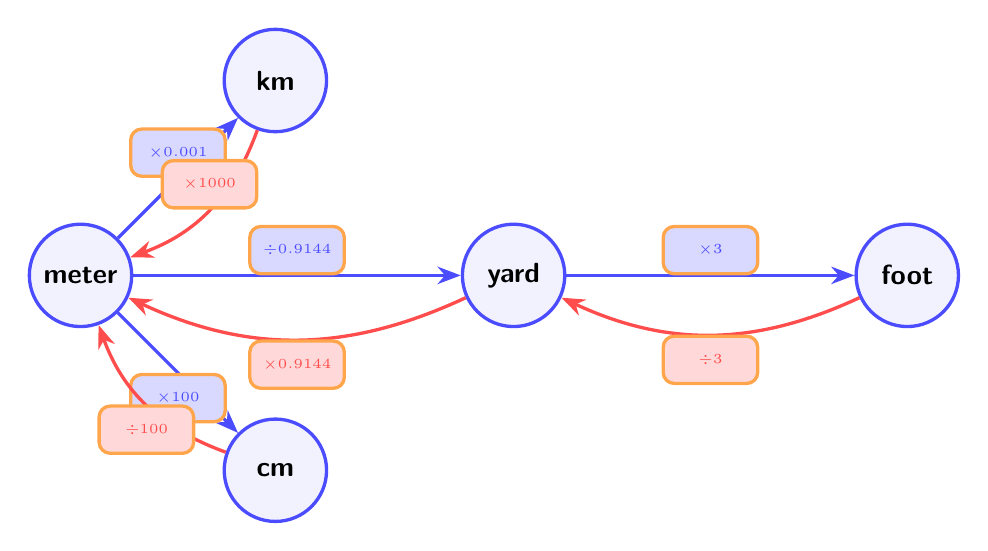
\begin{tikzpicture}[
  node distance=3.5cm and 4cm,
  unit/.style={circle, draw=blue!70, very thick, minimum size=1.3cm, font=\sffamily\bfseries, fill=blue!5},
  conversion/.style={rectangle, rounded corners, draw=orange!70, very thick, minimum width=1.2cm, minimum height=0.6cm, font=\tiny\sffamily, fill=orange!5},
  edge/.style={-Stealth, very thick}
]
  % Units (circles)
  \node[unit] (m) {meter};
  \node[unit, above right of=m] (km) {km};
  \node[unit, below right of=m] (cm) {cm};
  \node[unit, right of=m, xshift=2cm] (yd) {yard};
  \node[unit, right of=yd, xshift=1.5cm] (ft) {foot};
  
  % Forward conversions (blue)
  \path[edge, blue!70]
    (m) edge node[above, conversion, fill=blue!15] {$\times 0.001$} (km)
    (m) edge node[below, conversion, fill=blue!15] {$\times 100$} (cm)
    (m) edge node[above, conversion, fill=blue!15] {$\div 0.9144$} (yd)
    (yd) edge node[above, conversion, fill=blue!15] {$\times 3$} (ft);
    
  % Reverse conversions (red)
  \path[edge, red!70]
    (km) edge[bend left=25] node[above, conversion, fill=red!15] {$\times 1000$} (m)
    (cm) edge[bend left=25] node[below, conversion, fill=red!15] {$\div 100$} (m)
    (yd) edge[bend left=25] node[below, conversion, fill=red!15] {$\times 0.9144$} (m)
    (ft) edge[bend left=25] node[below, conversion, fill=red!15] {$\div 3$} (yd);
\end{tikzpicture}
\caption{Simple directed graph showing length unit conversions. Circle nodes represent units. Rectangular boxes represent conversion factors. Blue edges represent forward conversions, red edges represent reverse conversions.}
\label{fig:simple_digraph}
\end{figure}

In Figure~\ref{fig:simple_digraph}, each node represents a unit, and directed edges encode conversion factors. Notice that edges are \emph{bidirectional}—both forward and reverse conversions exist.

\subsection{Graphs vs. Lookup Tables}

\begin{table}[h]
\centering
\begin{tabular}{@{}lll@{}}
\toprule
\textbf{Feature} & \textbf{Lookup Table} & \textbf{Graph Network} \\
\midrule
Add 1 unit & Define $n$ conversions & Define $1{-}2$ edges \\
Storage & $O(n^2)$ & $O(n)$ or $O(n \log n)$ \\
Query time & $O(1)$ & $O(n)$ with caching $\rightarrow O(1)$ \\
Compound units & Exponential explosion & Compositional \\
Maintenance & Duplicate definitions & Canonical paths \\
Extensibility & Rigid & Dynamic \\
\bottomrule
\end{tabular}
\caption{Comparison of lookup tables vs. graph-based conversion}
\label{tab:graph_vs_lookup}
\end{table}

The key advantage: adding a new unit to a graph requires connecting it to \emph{one or two} existing units (e.g., connecting a new length unit only to \texttt{meter}), whereas a lookup table requires defining conversions to \emph{all} existing units.

\section{unyts Implementation}

\subsection{The UNode Class}

Each unit in the network is represented by a \texttt{UNode} object:

\begin{lstlisting}[style=pythonstyle, caption={UNode implementation (simplified)}]
class UNode:
    __slots__ = ('name',)
    
    def __init__(self, name: str):
        self.name = name
    
    def __eq__(self, other):
        return self.name == other.name
    
    def __hash__(self):
        return hash(self.name)
\end{lstlisting}

Key design choices:
\begin{itemize}[leftmargin=*]
  \item \textbf{Equality based on name}: Nodes created in different sessions compare equal
  \item \textbf{Hashable}: Enables use as dictionary keys for search memory caching
  \item \textbf{Lightweight}: Minimal memory footprint with \texttt{\_\_slots\_\_}
\end{itemize}

\subsection{The Conversion Class}

Directed edges encode transformation functions:

\begin{lstlisting}[style=pythonstyle, caption={Conversion class structure}]
class Conversion:
    def __init__(self, source: UNode, target: UNode, 
                 function: callable):
        self.source = source
        self.target = target
        self.function = function
\end{lstlisting}

A conversion from meters to kilometers stores:
\begin{lstlisting}[style=pythonstyle]
meter_to_km = Conversion(
    source=UNode('meter'),
    target=UNode('kilometer'),
    function=lambda x: x * 0.001
)
\end{lstlisting}

\subsection{The UDigraph Class}

The master graph object manages the entire network:

\begin{lstlisting}[style=pythonstyle, caption={UDigraph core attributes}]
class UDigraph:
    def __init__(self):
        self.edges = {}  # {UNode: ([children], [conversions])}
        self.memory = {} # Cached search results
        self.fvf = None  # Formation volume factor
    
    def add_node(self, node: UNode):
        if node not in self.edges:
            self.edges[node] = ([], [])
    
    def add_edge(self, conversion: Conversion):
        source = conversion.source
        if source not in self.edges:
            self.add_node(source)
        children, conversions = self.edges[source]
        children.append(conversion.target)
        conversions.append(conversion.function)
    
    def children_of(self, node: UNode):
        return self.edges[node][0] if node in self.edges else []
\end{lstlisting}

The \texttt{edges} dictionary maps each node to a tuple of \texttt{(child\_nodes, conversion\_functions)}, enabling efficient traversal during search.

\subsection{Building the Network}

Unit conversions are defined based on official standards:

\begin{lstlisting}[style=pythonstyle, caption={Example network construction}]
network = UDigraph()

# Define nodes
meter = UNode('meter')
kilometer = UNode('kilometer')
yard = UNode('yard')
foot = UNode('foot')

network.add_node(meter)
network.add_node(kilometer)
network.add_node(yard)
network.add_node(foot)

# Define conversions (both directions)
network.add_edge(Conversion(meter, kilometer, 
                           lambda x: x * 0.001))
network.add_edge(Conversion(kilometer, meter, 
                           lambda x: x * 1000))
network.add_edge(Conversion(meter, yard, 
                           lambda x: x / 0.9144))
network.add_edge(Conversion(yard, meter, 
                           lambda x: x * 0.9144))
network.add_edge(Conversion(yard, foot, 
                           lambda x: x * 3))
network.add_edge(Conversion(foot, yard, 
                           lambda x: x / 3))
\end{lstlisting}

\section{Why Graphs Win}

\subsection{Automatic Path Discovery}

Once the network is built, conversions between \emph{any} compatible unit pair are automatic. To convert 100 centimeters to feet:
\begin{enumerate}[leftmargin=*]
  \item BFS finds path: \texttt{cm} $\rightarrow$ \texttt{m} $\rightarrow$ \texttt{yard} $\rightarrow$ \texttt{foot}
  \item Apply transformations: $100 \div 100 \times (1/0.9144) \times 3 = 3.281$ feet
  \item Cache result for future use
\end{enumerate}

No explicit \texttt{cm} $\rightarrow$ \texttt{foot} conversion was ever defined!

\subsection{Bidirectional Conversion}

Every conversion automatically works in both directions. Defining \texttt{meter} $\rightarrow$ \texttt{yard} and its inverse enables conversions in either direction plus all transitive paths (meter $\rightarrow$ yard $\rightarrow$ foot).

\subsection{Composability}

Compound units emerge naturally:
\begin{itemize}[leftmargin=*]
  \item \texttt{kg/m3} decomposes to \texttt{kg} and \texttt{m3}
  \item Each component converts independently
  \item \texttt{stb/day/psi} = (standard barrels) / (day) / (pounds per square inch)
\end{itemize}

The graph handles numerator and denominator units separately, then recombines.

\subsection{Extensibility}

Adding industry-specific units requires minimal changes:

\begin{lstlisting}[style=pythonstyle, caption={Adding custom units}]
from unyts import set_unit, set_conversion

# Add a custom unit
set_unit('my_unit')

# Define conversion to an existing unit
set_conversion('my_unit', 'meter', 
               lambda x: x * 42.0,
               lambda x: x / 42.0)
\end{lstlisting}

The new unit immediately participates in all graph search operations, enabling conversions to \emph{any} compatible unit without additional definitions.

\section{Summary}

The directed graph architecture provides:
\begin{enumerate}[leftmargin=*]
  \item \textbf{Scalability}: $O(n)$ storage vs. $O(n^2)$ lookup tables
  \item \textbf{Maintainability}: Canonical definitions prevent inconsistencies
  \item \textbf{Flexibility}: Automatic discovery of conversion paths
  \item \textbf{Composability}: Natural handling of compound units
  \item \textbf{Extensibility}: Add units without modifying existing network
\end{enumerate}

The next chapter explores the graph search algorithms that traverse this network efficiently.


% ============================================================
% CHAPTER 3: SEARCH ALGORITHMS
% ============================================================
\chapter{Search Algorithms}

\texttt{unyts} implements four specialized graph search algorithms, each optimized for different conversion scenarios. This chapter explains their operation, performance characteristics, and use cases.

\section{Breadth-First Search (BFS)}

\subsection{Algorithm Overview}

BFS explores the graph \textbf{layer by layer}, visiting all nodes at distance $d$ before exploring nodes at distance $d+1$. This guarantees finding the \textbf{shortest path} between two nodes.

\textbf{Key properties}:
\begin{itemize}[leftmargin=*]
  \item \textbf{Completeness}: Finds a path if one exists
  \item \textbf{Optimality}: Always returns the shortest path
  \item \textbf{Time complexity}: $O(|V| + |E|)$ where $V$ = nodes, $E$ = edges
  \item \textbf{Space complexity}: $O(|V|)$ for the queue and visited set
\end{itemize}

\subsection{Implementation}

\begin{lstlisting}[style=pythonstyle, caption={BFS pseudocode}]
def BFS(graph, start, end):
    path_queue = [[start]]    # Queue of paths
    visited = []              # Visited paths
    
    while path_queue:
        current_path = path_queue.pop(0)  # Dequeue
        last_node = current_path[-1]
        
        if current_path in visited:
            continue
        visited.append(current_path)
        
        if last_node == end:
            return current_path  # Found!
        
        # Expand to children
        for child in graph.children_of(last_node):
            if child not in current_path:
                new_path = current_path + [child]
                path_queue.append(new_path)
    
    return None  # No path found
\end{lstlisting}

\subsection{Visual Example}

\begin{figure}[h]
\centering
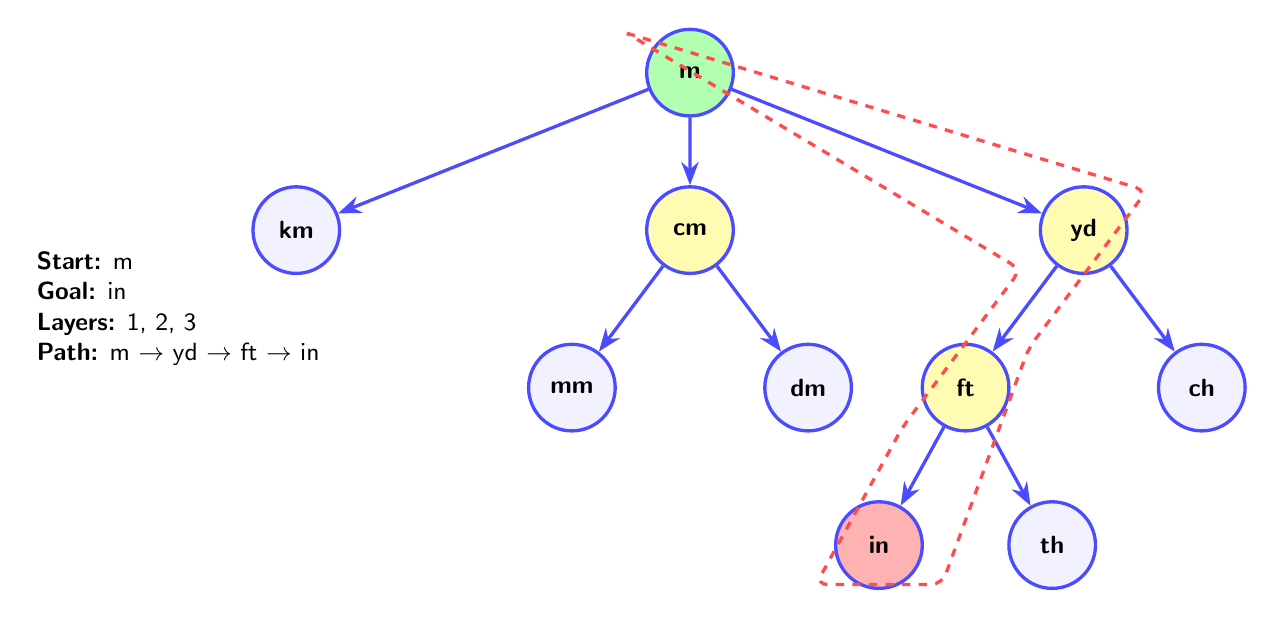
\begin{tikzpicture}[
  level distance=2cm,
  level 1/.style={sibling distance=5cm},
  level 2/.style={sibling distance=3cm},
  level 3/.style={sibling distance=2.2cm},
  every node/.style={circle, draw=blue!70, very thick, font=\small\sffamily\bfseries, minimum size=1.1cm, fill=blue!5},
  edge from parent/.style={draw, -Stealth, very thick, blue!70}
]
  \node[fill=green!30] (start) {m}
    child {node {km}}
    child {node[fill=yellow!30] (cm) {cm}
      child {node {mm}}
      child {node {dm}}
    }
    child {node[fill=yellow!30] (yd) {yd}
      child {node[fill=yellow!30] (ft) {ft}
        child {node[fill=red!30] (in) {in}}
        child {node {th}}
      }
      child {node {ch}}
    };
  
  \draw[dashed, very thick, red!70, rounded corners] 
    ($(start) + (-0.8, 0.5)$) -- ($(yd) + (0.8, 0.5)$) -- 
    ($(ft) + (0.8, 0.5)$) -- ($(in) + (0.8, -0.5)$) --
    ($(in) + (-0.8, -0.5)$) -- ($(ft) + (-0.8, -0.5)$) --
    ($(yd) + (-0.8, -0.5)$) -- ($(start) + (-0.8, 0.5)$);
  
  \node[rectangle, draw=none, fill=none, font=\small\sffamily, align=left] at (-6.5, -3) 
    {\textbf{Start:} m \\ \textbf{Goal:} in \\ \textbf{Layers:} 1, 2, 3 \\ \textbf{Path:} m {$\to$} yd {$\to$} ft {$\to$} in};
\end{tikzpicture}
\caption{BFS exploration tree. Green node is start, yellow nodes explored before red goal node (in). Dashed red line shows shortest path found. All unit nodes are circles.}
\label{fig:bfs_tree}
\end{figure}

In Figure~\ref{fig:bfs_tree}, BFS explores level 1 (km, cm, yd), then level 2 (mm, dm, ft, ch), discovering the shortest 3-hop path: meter → yard → foot → inch.

\subsection{Use Cases}

\begin{itemize}[leftmargin=*]
  \item When shortest conversion path is required
  \item Unknown network topology
  \item Verification of conversion accuracy
  \item Teaching/debugging conversion logic
\end{itemize}

\section{Depth-First Search (DFS)}

\subsection{Algorithm Overview}

DFS explores as \textbf{deep} as possible along each branch before backtracking. It uses \textbf{descendant filtering} to avoid exploring branches that cannot reach the goal.

\textbf{Key properties}:
\begin{itemize}[leftmargin=*]
  \item \textbf{Completeness}: Finds a path (but not necessarily shortest)
  \item \textbf{Optimality}: \emph{No} guarantee of shortest path
  \item \textbf{Time complexity}: $O(|V| + |E|)$ with pruning
  \item \textbf{Space complexity}: $O(|V|)$ for recursion stack
  \item \textbf{Advantage}: Often faster for deep paths
\end{itemize}

\subsection{Implementation with Descendant Filtering}

The \texttt{unyts} DFS implementation adds intelligent pruning:

\begin{lstlisting}[style=pythonstyle, caption={DFS with descendant filtering}]
def DFS(graph, start, end, branch_depth=25):
    def dfs_recursive(node, visited, path):
        visited.add(node)
        
        for child in graph.children_of(node):
            if child in visited:
                continue
            
            # Pruning: skip if goal unreachable within depth
            if end not in get_descendants(child, branch_depth):
                continue
            
            new_path = path + [child]
            
            if child == end:
                return new_path  # Found!
            
            result = dfs_recursive(child, visited, new_path)
            if end in result:
                return result
        
        return path
    
    return dfs_recursive(start, set(), [start])
\end{lstlisting}

The \texttt{get\_descendants(node, depth)} function precomputes all nodes reachable within \texttt{depth} hops, preventing exploration of dead-end branches.

\subsection{Visual Example}

\begin{figure}[h]
\centering
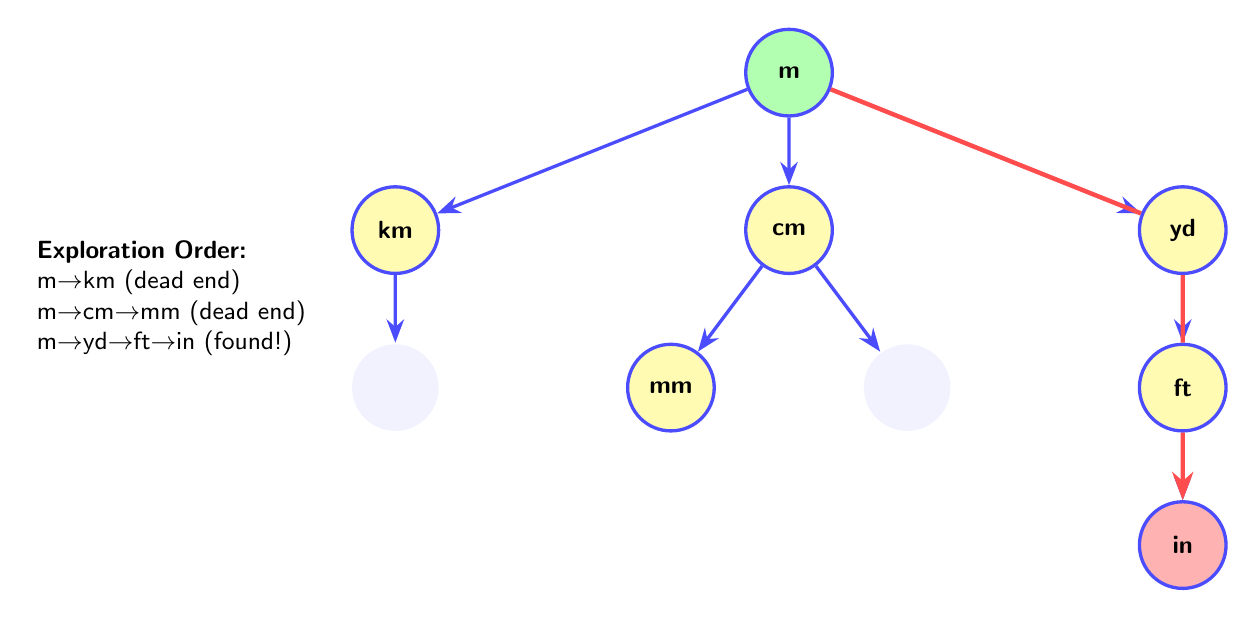
\begin{tikzpicture}[
  level distance=2cm,
  level 1/.style={sibling distance=5cm},
  level 2/.style={sibling distance=3cm},
  every node/.style={circle, draw=blue!70, very thick, font=\small\sffamily\bfseries, minimum size=1.1cm, fill=blue!5},
  edge from parent/.style={draw, -Stealth, very thick, blue!70}
]
  \node[fill=green!30] (start) {m}
    child {node[fill=yellow!30] {km}
      child {node[draw=none, font=\tiny] {}}
    }
    child {node[fill=yellow!30] {cm}
      child {node[fill=yellow!30] {mm}}
      child {node[draw=none, font=\tiny] {}}
    }
    child {node[fill=yellow!30] (yd) {yd}
      child {node[fill=yellow!30] (ft) {ft}
        child {node[fill=red!30] (in) {in}}
      }
    };
  
  \draw[ultra thick, red!70, -Stealth] (start) -- (yd) -- (ft) -- (in);
  \node[rectangle, draw=none, fill=none, font=\small\sffamily, align=left, anchor=north east] at (-6, -2) 
    {\textbf{Exploration Order:} \\ m{$\to$}km (dead end) \\ m{$\to$}cm{$\to$}mm (dead end) \\ m{$\to$}yd{$\to$}ft{$\to$}in (found!)};
\end{tikzpicture}
\caption{DFS exploration tree. Thick red arrows show the path DFS follows. Yellow nodes explored before finding goal. All unit nodes are circles.}
\label{fig:dfs_tree}
\end{figure}

DFS may explore fewer nodes than BFS if the goal happens to be on the first deep branch explored (though it might also explore more if unlucky).

\subsection{Use Cases}

\begin{itemize}[leftmargin=*]
  \item Known deep conversion paths (e.g., complex compound units)
  \item Memory-constrained environments
  \item When first valid path is acceptable
\end{itemize}

\section{lean\_BFS (Optimized BFS)}

\subsection{Innovation: Network Pruning}

The classic BFS bottleneck is exploring nodes irrelevant to the start→end conversion. \textbf{lean\_BFS} addresses this by:
\begin{enumerate}[leftmargin=*]
  \item Compute descendants of \texttt{start} up to depth $d$: $D_{start}$
  \item Compute descendants of \texttt{end} up to depth $d$: $D_{end}$
  \item Find intersection: $D_{relevant} = D_{start} \cap D_{end}$
  \item Construct \textbf{slimmed network} containing only nodes in $D_{relevant}$
  \item Run standard BFS on this smaller network
\end{enumerate}

\subsection{Multi-Generation Strategy}

lean\_BFS iteratively tries increasing depths: $[0, 1, 2, 3, 4, 5, 7, 10, 13, 16, 20, 25, \ldots]$ until the intersection is non-empty. This avoids over-expanding for simple conversions while handling complex ones.

\begin{lstlisting}[style=pythonstyle, caption={lean\_BFS network filtering}]
def lean_BFS(graph, start, end, max_gen=25):
    generations = [0, 1, 2, 3, 4, 5, 7, 10, 13, 16, 20, 25]
    
    for depth in generations:
        if depth > max_gen:
            break
        
        start_desc = get_descendants(start, depth)
        end_desc = get_descendants(end, depth)
        intersection = start_desc & end_desc
        
        if intersection:
            # Build slim network with only these nodes
            slim_edges = {
                node: graph.edges[node] 
                for node in intersection 
                if node in graph.edges
            }
            slim_graph = SlimUDigraph(slim_edges)
            return BFS(slim_graph, start, end)
    
    return None  # No path found
\end{lstlisting}

\subsection{Performance Gains}

Typical performance improvement over standard BFS:
\begin{itemize}[leftmargin=*]
  \item \textbf{Network size reduction}: From 500+ nodes to 10–30 relevant nodes
  \item \textbf{Speed improvement}: 5–20× faster for typical conversions
  \item \textbf{Memory savings}: Proportional to network reduction
\end{itemize}

\subsection{Use Cases}

\begin{itemize}[leftmargin=*]
  \item \textbf{Default algorithm} for most conversions
  \item Production systems requiring fast response
  \item Repeated conversions between popular unit pairs
\end{itemize}

\section{hybrid\_BFS (Parallel Search)}

\subsection{Concurrent Execution}

hybrid\_BFS runs \textbf{BFS and lean\_BFS simultaneously} in separate threads (or processes), returning the first successful result:

\begin{lstlisting}[style=pythonstyle, caption={hybrid\_BFS parallel execution}]
def hybrid_BFS(graph, start, end):
    results = {'bfs': '', 'lean_bfs': ''}
    
    thread_bfs = Thread(target=run_bfs, 
                       args=(results, graph, start, end))
    thread_lean = Thread(target=run_lean_bfs, 
                        args=(results, graph, start, end))
    
    thread_bfs.start()
    thread_lean.start()
    
    while True:
        if results['lean_bfs']:
            thread_bfs.terminate()
            return results['lean_bfs']
        elif results['bfs']:
            thread_lean.terminate()
            return results['bfs']
        elif results['bfs'] is None and results['lean_bfs'] is None:
            return None  # Both failed
\end{lstlisting}

\subsection{Parallelization Options}

\texttt{unyts} supports multiple parallel backends:
\begin{itemize}[leftmargin=*]
  \item \textbf{Threading}: Default for Python <3.13 (GIL-limited)
  \item \textbf{Multiprocessing}: Python 3.14+ with free-threading (true parallelism)
  \item \textbf{Auto}: Automatically selects best available method
\end{itemize}

\subsection{Use Cases}

\begin{itemize}[leftmargin=*]
  \item Unknown path complexity
  \item Time-critical conversions
  \item Multi-core systems
  \item When willing to trade CPU for speed
\end{itemize}

\section{Algorithm Comparison}

\begin{table}[h]
\centering
\begin{tabular}{@{}lcccc@{}}
\toprule
\textbf{Algorithm} & \textbf{Shortest Path} & \textbf{Speed} & \textbf{Memory} & \textbf{Best For} \\
\midrule
BFS & Yes & Medium & High & Shortest guarantee \\
DFS & No & Fast (deep) & Low & Known deep paths \\
lean\_BFS & Yes & Fast & Medium & Most conversions \\
hybrid\_BFS & Yes & Fastest & Highest & Critical speed \\
\bottomrule
\end{tabular}
\caption{Search algorithm comparison}
\label{tab:algorithm_comparison}
\end{table}

\subsection{Selection Guidelines}

\begin{itemize}[leftmargin=*]
  \item \textbf{Default}: Use \texttt{lean\_BFS} (fast + optimal)
  \item \textbf{Verification}: Use \texttt{BFS} to confirm shortest path
  \item \textbf{Complex units}: Try \texttt{DFS} for deep compound ratios
  \item \textbf{Maximum speed}: Use \texttt{hybrid\_BFS} with multiprocessing
\end{itemize}

The algorithm can be changed globally or per-conversion:

\begin{lstlisting}[style=pythonstyle]
import unyts

# Set globally
unyts.set_algorithm('hybrid_BFS')

# All conversions use hybrid_BFS from now on
result = convert(100, 'cm', 'in')
\end{lstlisting}

\section{Summary}

\texttt{unyts} provides four specialized search algorithms, each optimized for different scenarios. The default \texttt{lean\_BFS} combines the shortest-path guarantee of BFS with network pruning for excellent performance. Users can select algorithms based on their specific needs: verification (BFS), deep paths (DFS), or maximum speed (hybrid\_BFS).


% ============================================================  
% CHAPTER 4: THE UNITS NETWORK
% ============================================================
\chapter{The Units Network}

This chapter explains how the unit conversion network is organized, how conversions are defined based on official standards, and visualizes key network segments.

\section{Network Organization Principles}

\subsection{Canonical Definitions}

Every unit conversion in \texttt{unyts} is based on \textbf{official international standards} or widely accepted definitions:

\begin{itemize}[leftmargin=*]
  \item \textbf{1 foot} = 12 inches (by definition)
  \item \textbf{1 yard} = 3 feet (by definition)
  \item \textbf{1 yard} = 0.9144 meters (exact, 1959 international yard)
  \item \textbf{1 kilometer} = 1000 meters (SI prefix definition)
  \item \textbf{1 pound} = 0.45359237 kilograms (exact, by definition)
\end{itemize}

This ensures consistency and prevents accumulation of rounding errors across multiple conversions.

\subsection{No Duplicate Paths}

A key design principle: between any two units, there exists \textbf{exactly one canonical conversion path}. This prevents:
\begin{itemize}[leftmargin=*]
  \item Conflicting conversion factors
  \item Cyclic dependencies with rounding errors
  \item Ambiguity in path selection
\end{itemize}

For example, to convert \texttt{foot} to \texttt{meter}, the path is uniquely:
\[
\text{foot} \rightarrow \text{yard} \rightarrow \text{meter}
\]

There is no direct \texttt{foot} $\rightarrow$ \texttt{meter} edge, ensuring all foot-to-meter conversions use the same computation.

\subsection{Modular Structure}

The network is organized into loosely-coupled modules:
\begin{enumerate}[leftmargin=*]
  \item \textbf{SI System}: Each base unit (meter, gram, second) connects to its SI prefixes
  \item \textbf{Imperial System}: Units form chains based on their definitions
  \item \textbf{Bridges}: Connect SI and Imperial systems at specific units
  \item \textbf{Specialized Systems}: Temperature, pressure gauges, oil field units
\end{enumerate}

\section{Length Network}

\subsection{SI Prefix Structure}

The meter serves as the SI base unit for length, with prefix multipliers defined by powers of 10:

\begin{figure}[h]
\centering
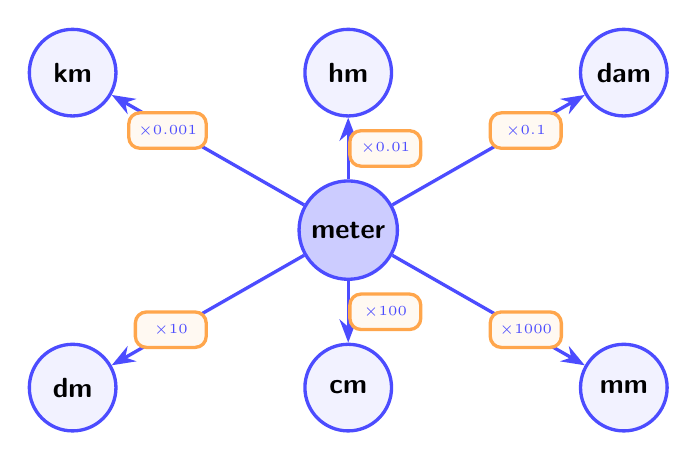
\begin{tikzpicture}[
  unit/.style={circle, draw=blue!70, very thick, font=\sffamily\bfseries, minimum size=1.1cm, fill=blue!5},
  conversion/.style={rectangle, rounded corners, draw=orange!70, very thick, minimum width=0.9cm, minimum height=0.45cm, font=\tiny\sffamily, fill=orange!5},
  >=Stealth
]
  % Center: meter
  \node[unit, fill=blue!20] (m) at (0, 0) {meter};
  
  % Top row: larger units (multiplier < 1)
  \node[unit] (km) at (-3.5, 2) {km};
  \node[unit] (hm) at (0, 2) {hm};
  \node[unit] (dam) at (3.5, 2) {dam};
  
  % Bottom row: smaller units (multiplier > 1)
  \node[unit] (dm) at (-3.5, -2) {dm};
  \node[unit] (cm) at (0, -2) {cm};
  \node[unit] (mm) at (3.5, -2) {mm};
  
  % Connections: meter to top row
  \path[-Stealth, very thick, blue!70]
    (m) edge node[conversion, above left] {$\times 0.001$} (km)
    (m) edge node[conversion, right] {$\times 0.01$} (hm)
    (m) edge node[conversion, above right] {$\times 0.1$} (dam);
  
  % Connections: meter to bottom row
  \path[-Stealth, very thick, blue!70]
    (m) edge node[conversion, below left] {$\times 10$} (dm)
    (m) edge node[conversion, right] {$\times 100$} (cm)
    (m) edge node[conversion, below right] {$\times 1000$} (mm);
\end{tikzpicture}
\caption{SI prefix network for length. Meter is the hub unit (blue center). Larger units above, smaller units below. All conversions route through the base unit. Circle nodes represent units, rectangular boxes represent conversion factors.}
\label{fig:si_length}
\end{figure}

Additional SI prefixes (micro, nano, pico, kilo, mega, giga, etc.) follow the same pattern. The meter acts as a \textbf{hub node} for the SI subsystem.

\subsection{Imperial Chain Structure}

Imperial units form a \textbf{linear chain} based on their historical definitions:

\begin{figure}[h]
\centering
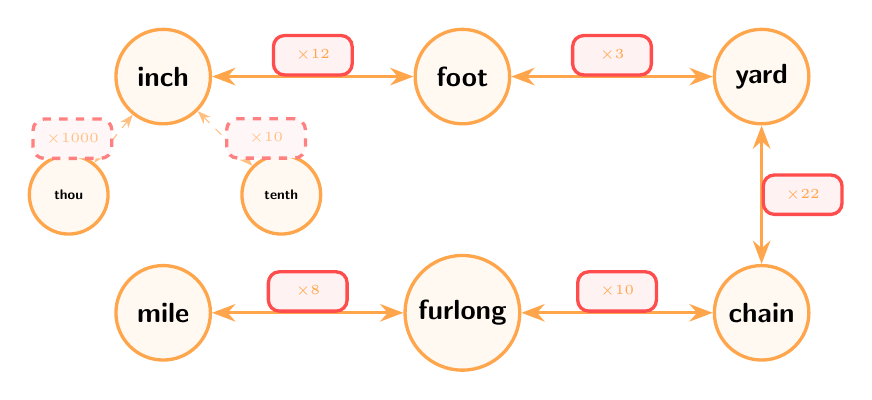
\begin{tikzpicture}[
  unit/.style={circle, draw=orange!70, very thick, minimum size=1.2cm, font=\sffamily\bfseries, fill=orange!5},
  conversion/.style={rectangle, rounded corners, draw=red!70, very thick, minimum width=1cm, minimum height=0.5cm, font=\tiny\sffamily, fill=red!5},
  >=Stealth
]
  % Row 1 (left to right): inch -> foot -> yard
  \node[unit] (in) at (0, 0) {inch};
  \node[unit] (ft) at (3.8, 0) {foot};
  \node[unit] (yd) at (7.6, 0) {yard};
  
  % Row 2 (right to left): chain <- furlong <- mile
  \node[unit] (ch) at (7.6, -3) {chain};
  \node[unit] (fur) at (3.8, -3) {furlong};
  \node[unit] (mi) at (0, -3) {mile};
  
  % Top row connections
  \path[<->, very thick, orange!70]
    (in) edge node[conversion, above] {$\times 12$} (ft)
    (ft) edge node[conversion, above] {$\times 3$} (yd);
  
  % S-bend: yard down to chain
  \path[<->, very thick, orange!70]
    (yd) edge node[conversion, right] {$\times 22$} (ch);
  
  % Bottom row connections (right to left)
  \path[<->, very thick, orange!70]
    (ch) edge node[conversion, above] {$\times 10$} (fur)
    (fur) edge node[conversion, above] {$\times 8$} (mi);
  
  % Sub-units (dashed)
  \node[unit, minimum size=1cm, font=\sffamily\bfseries\tiny] (th) at (-1.2, -1.5) {thou};
  \node[unit, minimum size=1cm, font=\sffamily\bfseries\tiny] (tenth) at (1.5, -1.5) {tenth};
  
  \path[<->, dashed, orange!50]
    (in) edge node[conversion, left, draw=red!50, fill=red!3] {$\times 1000$} (th)
    (in) edge node[conversion, right, draw=red!50, fill=red!3] {$\times 10$} (tenth);
\end{tikzpicture}
\caption{Imperial length chain (S-shaped layout). Top row flows left to right (inch{$\to$}foot{$\to$}yard), then wraps down to bottom row right to left (chain{$\to$}furlong{$\to$}mile). Circle nodes represent units, rectangular boxes represent conversion factors. Dashed lines show fractional sub-units.}
\label{fig:imperial_chain}
\end{figure}

\subsection{SI-Imperial Bridge}

The two systems connect at a single point: \textbf{yard ↔ meter}

\begin{figure}[h]
\centering
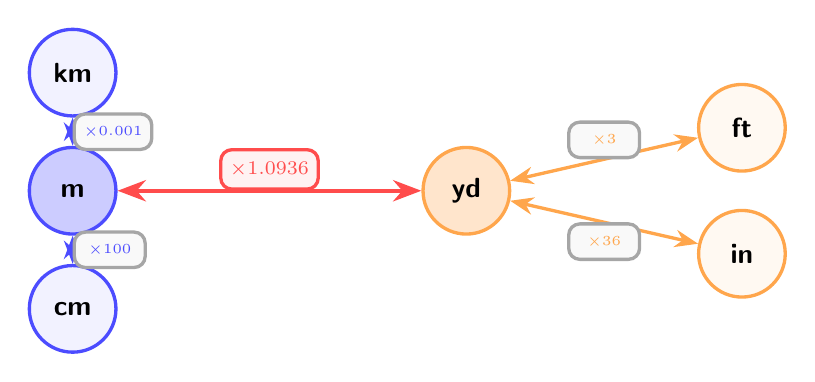
\begin{tikzpicture}[
  sunit/.style={circle, draw=blue!70, very thick, minimum size=1.1cm, font=\sffamily\bfseries, fill=blue!5},
  iunit/.style={circle, draw=orange!70, very thick, minimum size=1.1cm, font=\sffamily\bfseries, fill=orange!5},
  conversion/.style={rectangle, rounded corners, draw=gray!70, very thick, minimum width=0.9cm, minimum height=0.45cm, font=\tiny\sffamily, fill=gray!5},
  bridge/.style={rectangle, rounded corners, draw=red!70, very thick, minimum width=1.2cm, minimum height=0.5cm, font=\scriptsize\sffamily\bfseries, fill=red!5},
  >=Stealth
]
  % SI side (left column)
  \node[sunit] (km) at (0, 1.5) {km};
  \node[sunit, fill=blue!20] (m) at (0, 0) {m};
  \node[sunit] (cm) at (0, -1.5) {cm};
  
  % Bridge connection (center)
  \node[iunit, fill=orange!20] (yd) at (5, 0) {yd};
  
  % Imperial side (right)
  \node[iunit] (ft) at (8.5, 0.8) {ft};
  \node[iunit] (in) at (8.5, -0.8) {in};
  
  % SI internal connections
  \path[<->, blue!70, very thick]
    (km) edge node[conversion, right] {$\times 0.001$} (m)
    (cm) edge node[conversion, right] {$\times 100$} (m);
  
  % Bridge (red, prominent)
  \path[<->, red!70, ultra thick]
    (m) edge node[bridge, above] {$\times 1.0936$} (yd);
  
  % Imperial connections
  \path[<->, orange!70, very thick]
    (yd) edge node[conversion, above] {$\times 3$} (ft)
    (yd) edge node[conversion, below] {$\times 36$} (in);
\end{tikzpicture}
\caption{The SI-Imperial bridge. SI units (blue, left) connect to Imperial units (orange, right) through the meter{$\leftrightarrow$}yard bridge (red). All cross-system conversions must route through this connection. Circle nodes represent units, rectangular boxes represent conversion factors.}
\label{fig:si_imperial_bridge}
\end{figure}

\subsection{Complete Length Network with Highlighted Path}

Figure~\ref{fig:length_network_full} shows the complete length network with a highlighted conversion path from \textbf{centimeter to inch}:

\begin{figure}[h]
\centering
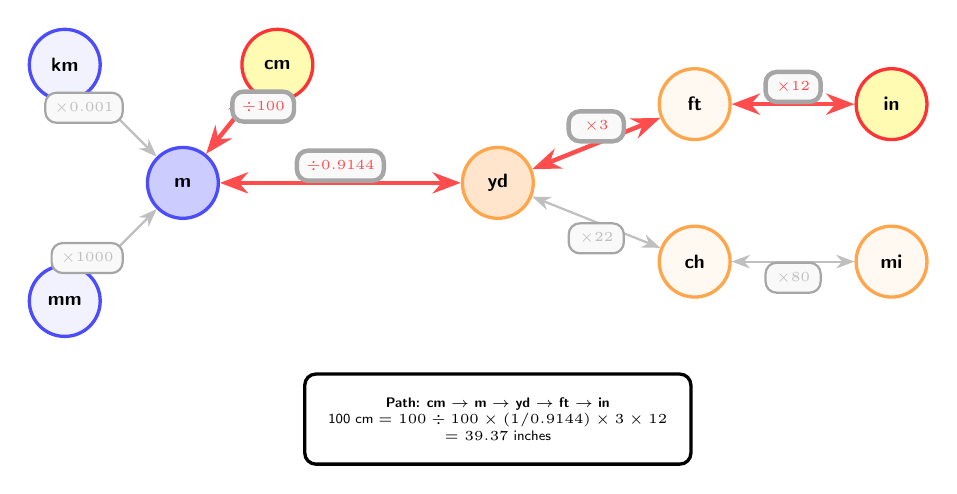
\begin{tikzpicture}[
  unit/.style={circle, draw=blue!70, very thick, minimum size=0.9cm, font=\scriptsize\sffamily\bfseries, fill=blue!5},
  iunit/.style={circle, draw=orange!70, very thick, minimum size=0.9cm, font=\scriptsize\sffamily\bfseries, fill=orange!5},
  highlight/.style={circle, draw=red!80, very thick, minimum size=0.9cm, font=\scriptsize\sffamily\bfseries, fill=yellow!30},
  conversion/.style={rectangle, rounded corners, draw=gray!70, minimum width=0.7cm, minimum height=0.35cm, font=\tiny\sffamily, fill=gray!5},
  standard/.style={<->, thick, gray!50},
  highlight_edge/.style={<->, ultra thick, red!70},
  >=Stealth
]
  % SI system (left)
  \node[unit, fill=blue!20] (m) at (0, 0) {m};
  \node[unit] (km) at (-1.5, 1.5) {km};
  \node[unit] (mm) at (-1.5, -1.5) {mm};
  \node[highlight] (cm) at (1.2, 1.5) {cm};
  
  % Bridge
  \node[iunit, fill=orange!20] (yd) at (4, 0) {yd};
  
  % Imperial system (right)
  \node[iunit] (ft) at (6.5, 1) {ft};
  \node[highlight] (in) at (9, 1) {in};
  \node[iunit] (ch) at (6.5, -1) {ch};
  \node[iunit] (mi) at (9, -1) {mi};
  
  % SI connections (gray)
  \path[standard]
    (m) edge node[conversion, above left] {$\times 0.001$} (km)
    (m) edge node[conversion, below left] {$\times 1000$} (mm);
  
  % Highlighted path: cm -> m -> yd -> ft -> in
  \path[highlight_edge]
    (cm) edge node[conversion, above right] {$\div 100$} (m)
    (m) edge node[conversion, above] {$\div 0.9144$} (yd)
    (yd) edge node[conversion, above] {$\times 3$} (ft)
    (ft) edge node[conversion, above] {$\times 12$} (in);
  
  % Imperial standard connections
  \path[standard]
    (yd) edge node[conversion, below] {$\times 22$} (ch)
    (ch) edge node[conversion, below] {$\times 80$} (mi);
  
  % Legend with full calculation
  \node[draw=black, very thick, rounded corners, fill=white, inner sep=0.3cm, font=\tiny\sffamily, align=center]
    at (4, -3) {\textbf{Path: cm {$\to$} m {$\to$} yd {$\to$} ft {$\to$} in} \\
     100 cm $= 100 \div 100 \times (1/0.9144) \times 3 \times 12$ \\
     $= 39.37$ inches};
\end{tikzpicture}
\caption{Complete length network showing highlighted conversion path from centimeter to inch (yellow nodes). Red thick arrows trace the conversion route. Gray connections show other available paths. Circle nodes represent units, rectangular boxes represent conversion factors.}
\label{fig:length_network_full}
\end{figure}

\section{Time Network}

The time network forms a \textbf{hierarchical tree} structure:

\begin{figure}[h]
\centering
\begin{tikzpicture}[
  level distance=1.6cm,
  level 1/.style={sibling distance=6.5cm},
  level 2/.style={sibling distance=3.5cm},
  level 3/.style={sibling distance=2cm},
  every node/.style={rectangle, rounded corners, draw, font=\small\sffamily, minimum width=1.1cm},
  every edge/.style={draw, <->, thick, teal!60}
]
  \node[fill=teal!20] {second}
    child {node {μs}
      edge from parent node[left, font=\tiny] {×1e6}
    }
    child {node {ms}
      edge from parent node[left, font=\tiny] {×1000}
    }
    child {node {minute}
      child {node {hour}
        child {node {day}
          child {node[fill=yellow!20] {week}
            edge from parent node[left, font=\tiny] {×7}
          }
          child {node[fill=yellow!20] {month}
            child {node {year}
              child {node {decade}}
              child {node {century}}
            }
            edge from parent node[right, font=\tiny] {×30.44}
          }
        }
      }
      edge from parent node[right, font=\tiny] {×60}
    };
\end{tikzpicture}
\caption{Time network hierarchical structure. Tree shows conversions from microseconds through seconds, minutes, hours, days to larger units. Yellow nodes (week, month) are alternatives branching from day.}
\label{fig:time_network}
\end{figure}

Note that \texttt{month} uses the average month length (30.4375 days) and conversions involving months are approximate. The year node connects to \texttt{day} (365.25 days) and \texttt{month} (12 months), providing both paths.

\section{Temperature Network}

Temperature conversions are \textbf{non-linear} due to offset + scale transformations:

\begin{figure}[h]
\centering
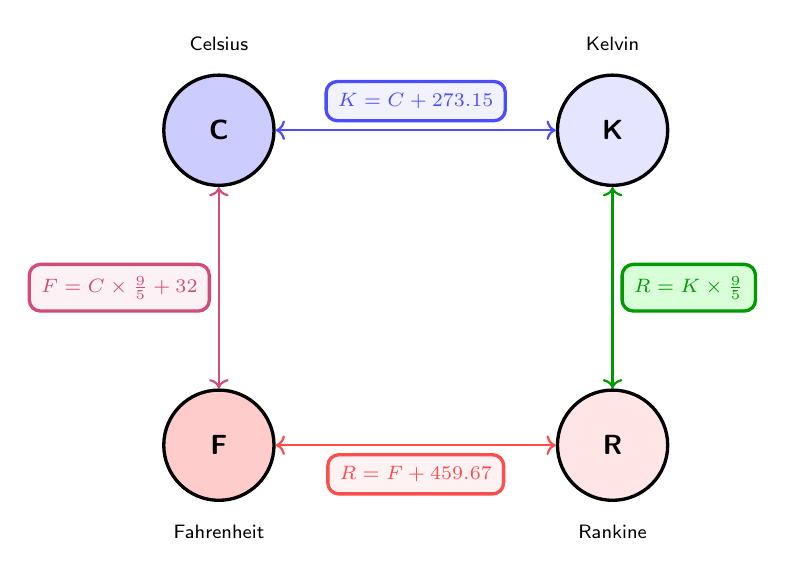
\begin{tikzpicture}[
  unit/.style={circle, draw, very thick, minimum size=1.4cm, font=\sffamily\bfseries, align=center},
  formula/.style={rectangle, rounded corners, draw, very thick, inner sep=0.15cm, font=\scriptsize},
  label/.style={rectangle, draw=none, fill=none, font=\scriptsize\sffamily},
  every edge/.style={draw, <->, thick}
]
  \node[unit, fill=blue!20] (C) at (0, 0) {C};
  \node[unit, fill=blue!10] (K) at (5, 0) {K};
  \node[unit, fill=red!20] (F) at (0, -4) {F};
  \node[unit, fill=red!10] (R) at (5, -4) {R};
  
  % Full names outside circles
  \node[label] at (0, 1.1) {Celsius};
  \node[label] at (5, 1.1) {Kelvin};
  \node[label] at (0, -5.1) {Fahrenheit};
  \node[label] at (5, -5.1) {Rankine};
  
  % Horizontal edges
  \path[blue!70]
    (C) edge node[formula, draw=blue!70, fill=blue!5, above, yshift=0.1cm] {$K = C + 273.15$} (K);
  \path[red!70]
    (F) edge node[formula, draw=red!70, fill=red!5, below, yshift=-0.1cm] {$R = F + 459.67$} (R);
  
  % Vertical edges
  \path[purple!70]
    (C) edge node[formula, draw=purple!70, fill=purple!5, left, xshift=-0.1cm] {$F = C \times \frac{9}{5} + 32$} (F);
  \path[green!60!black]
    (K) edge node[formula, draw=green!60!black, fill=green!15, right, xshift=0.1cm] {$R = K \times \frac{9}{5}$} (R);
\end{tikzpicture}
\caption{Temperature network showing all bidirectional conversions in rectangular boxes. Each conversion encodes both offset and scale transformations. Circle nodes represent temperature scales, rectangular boxes show conversion formulas.}
\label{fig:temperature_network}
\end{figure}

The conversion functions for temperature include both multiplication and addition:
\begin{lstlisting}[style=pythonstyle, caption={Temperature conversion example}]
Celsius_to_Fahrenheit = lambda C: C * 9/5 + 32
Fahrenheit_to_Celsius = lambda F: (F - 32) * 5/9
\end{lstlisting}

\section{Other Network Segments}

\subsection{Volume Network}

Volume conversions split into three subsystems:
\begin{itemize}[leftmargin=*]
  \item \textbf{Cubic units}: $\text{m}^3$, $\text{cm}^3$, $\text{ft}^3$, $\text{in}^3$ (derived from length)
  \item \textbf{Liquid volume (US)}: gallon → quart → pint → gill → fluid ounce
  \item \textbf{Liquid volume (UK)}: Imperial gallon → quart → pint (different definitions than US)
  \item \textbf{Bridge}: Liter ↔ $\text{cm}^3$ (exact), gallon(UK) ↔ liter, gallon(US) ↔ cubic inch
\end{itemize}

\subsection{Pressure Network}

Pressure includes both absolute and gauge measurements:
\begin{itemize}[leftmargin=*]
  \item \textbf{Absolute}: Pascal (Pa), bar, psi(a), atmosphere, Torr
  \item \textbf{Gauge}: barg ↔ bara (offset by atmospheric pressure), psig ↔ psia
  \item \textbf{Conversions}: bar ↔ Pascal ↔ atmosphere, psi ↔ bar
\end{itemize}

\subsection{Mass Network}

Similar to length, mass has SI (gram-based) and Imperial (pound-based) subsystems:
\begin{itemize}[leftmargin=*]
  \item \textbf{SI}: kilogram → gram (with prefixes: mg, kg, tonne)
  \item \textbf{Imperial}: pound → ounce → dram, ton → hundredweight → stone → quarter
  \item \textbf{Bridge}: pound ↔ kilogram (exact conversion)
\end{itemize}

\section{Example Conversion Walkthrough}

Let's trace the conversion of \textbf{100 centimeters to inches} step by step:

\subsection{Step 1: Find Path}

lean\_BFS searches and finds:
\[
\texttt{cm} \rightarrow \texttt{m} \rightarrow \texttt{yard} \rightarrow \texttt{foot} \rightarrow \texttt{inch}
\]

\subsection{Step 2: Apply Transformations}

\begin{align*}
\text{cm} &\rightarrow \text{m}: \quad && 100 \div 100 = 1.0 \text{ meter} \\
\text{m} &\rightarrow \text{yard}: \quad && 1.0 \div 0.9144 = 1.0936 \text{ yards} \\
\text{yard} &\rightarrow \text{foot}: \quad && 1.0936 \times 3 = 3.2808 \text{ feet} \\
\text{foot} &\rightarrow \text{inch}: \quad && 3.2808 \times 12 = 39.37 \text{ inches}
\end{align*}

\subsection{Step 3: Cache Result}

The conversion path and final multiplier ($39.37 / 100 = 0.3937$) are cached:
\begin{lstlisting}[style=pythonstyle]
units_network.memory[('cm', 'inch')] = {
    'path': ['cm', 'm', 'yard', 'foot', 'inch'],
    'factor': 0.3937
}
\end{lstlisting}

Future \texttt{cm} → \texttt{inch} conversions retrieve this cached result instantly ($O(1)$ lookup).

\section{Summary}

The \texttt{unyts} network is carefully organized around:
\begin{enumerate}[leftmargin=*]
  \item \textbf{Official definitions}: All conversions based on international standards
  \item \textbf{Single canonical paths}: No duplicate routes between unit pairs
  \item \textbf{Modular structure}: SI, Imperial, and specialized subsystems
  \item \textbf{Strategic bridges}: Minimal connections between subsystems
  \item \textbf{Hub topology}: Base units (meter, gram, second) serve as central nodes
\end{enumerate}

This architecture enables automatic discovery of conversion paths for thousands of unit combinations from a compact set of defining relationships.


% ============================================================
% CHAPTER 5: INSTALLATION
% ============================================================
\chapter{Installation}

\section{Requirements}

\subsection{Python Version}
\texttt{unyts} supports Python 3.7 and later. The package metadata targets:
\begin{lstlisting}[style=bashstyle]
requires-python = ">=3.7"
\end{lstlisting}

Recommended: Python 3.10+ for optimal performance.

\subsection{Core Dependencies}

Required packages (automatically installed with \texttt{unyts}):
\begin{itemize}[leftmargin=*]
  \item \texttt{stringthings}: Helper utilities for string processing
  \item \texttt{cloudpickle}: Caching network and search memory
\end{itemize}

\subsection{Optional Dependencies}

While not required, the following packages enhance \texttt{unyts} functionality:
\begin{itemize}[leftmargin=*]
  \item \textbf{NumPy}: Enables array-aware conversions, handles lists/ndarrays
  \item \textbf{Pandas}: Recognizes Series/DataFrame objects for bulk conversions
  \item \textbf{openpyxl}: Required only for exporting the network to Excel format
\end{itemize}

Install optional dependencies manually if needed:
\begin{lstlisting}[style=bashstyle]
pip install numpy pandas openpyxl
\end{lstlisting}

\section{Installation Methods}

\subsection{Install from PyPI (Recommended)}

The simplest installation method:
\begin{lstlisting}[style=bashstyle]
pip install unyts
\end{lstlisting}

\subsection{Upgrade to Latest Version}

To ensure you have the latest features and bug fixes:
\begin{lstlisting}[style=bashstyle]
pip install --upgrade unyts
\end{lstlisting}

\subsection{Install from Source}

For development or testing unreleased features:
\begin{lstlisting}[style=bashstyle]
git clone https://github.com/ayaranitram/unyts.git
cd unyts
pip install -e .
\end{lstlisting}

The \texttt{-e} flag installs in editable mode, allowing you to modify source code and see changes immediately.

\section{Verification}

Verify the installation by checking the version:

\begin{lstlisting}[style=pythonstyle]
import unyts
print(unyts.__version__)  # Should print: 0.10.1 (or later)
\end{lstlisting}

Test basic functionality:

\begin{lstlisting}[style=pythonstyle]
from unyts import convert

result = convert(1, 'meter', 'foot')
print(result)  # Should print: 3.280839895013123
\end{lstlisting}

If no errors occur, \texttt{unyts} is correctly installed and operational.

\section{First-Time Setup}

On first import, \texttt{unyts} performs one-time initialization:
\begin{enumerate}[leftmargin=*]
  \item Builds the unit conversion network from definitions
  \item Loads search memory cache (if available)
  \item Creates user configuration directory
\end{enumerate}

This process may take a few seconds. Subsequent imports are faster due to caching.

\section{Configuration Files}

\texttt{unyts} stores configuration and cache files in a user-specific directory:
\begin{itemize}[leftmargin=*]
  \item \textbf{Windows}: \texttt{C:\textbackslash Users\textbackslash<username>\textbackslash .unyts\textbackslash}
  \item \textbf{macOS/Linux}: \texttt{\textasciitilde/.unyts/}
\end{itemize}

Files stored:
\begin{itemize}[leftmargin=*]
  \item \texttt{parameters.ini}: User preferences (algorithm, print path, etc.)
  \item \texttt{search\_memory.cache}: Cached conversion paths
  \item \texttt{units\_network.cache}: Serialized network (future optimization)
\end{itemize}

To reset \texttt{unyts} to defaults, delete this directory and re-import.

\section{Troubleshooting Installation}

\subsection{Missing cloudpickle}

If you see warnings about cloudpickle:
\begin{lstlisting}[style=bashstyle]
Warning: Missing `cloudpickle` package. 
Not able to cache search memory.
\end{lstlisting}

Install it explicitly:
\begin{lstlisting}[style=bashstyle]
pip install cloudpickle
\end{lstlisting}

\subsection{Import Errors}

If imports fail with \texttt{ModuleNotFoundError}, ensure \texttt{unyts} is installed in the active Python environment:
\begin{lstlisting}[style=bashstyle]
pip list | grep unyts
\end{lstlisting}

If using virtual environments or conda, activate the correct environment before installation.

\subsection{Version Conflicts}

If upgrading causes issues, completely remove the old version first:
\begin{lstlisting}[style=bashstyle]
pip uninstall unyts
pip install unyts
\end{lstlisting}


% ============================================================
% CHAPTER 6: QUICK START
% ============================================================
\chapter{Quick Start}

This chapter provides a concise introduction to using \texttt{unyts} for common tasks.

\section{Basic Conversion}

The simplest way to use \texttt{unyts} is via the \texttt{convert()} function:

\begin{lstlisting}[style=pythonstyle]
from unyts import convert

# Convert 10 feet to meters
meters = convert(10, 'ft', 'm')
print(meters)  # Output: 3.048
\end{lstlisting}

The function signature is:
\begin{lstlisting}[style=pythonstyle]
convert(value, from_units, to_units, 
        print_conversion_path=None, use_cache=True)
\end{lstlisting}

\begin{itemize}[leftmargin=*]
  \item \texttt{value}: Numeric input (int, float, list, np.array, pd.Series)
  \item \texttt{from\_units}: Source unit string (e.g., \texttt{'ft'}, \texttt{'kg/m3'})
  \item \texttt{to\_units}: Target unit string
  \item \texttt{print\_conversion\_path}: Override global print\_path setting
  \item \texttt{use\_cache}: Set \texttt{False} to force fresh search
\end{itemize}

\section{Creating Unit-Aware Quantities}

Use the \texttt{units()} factory function to create \texttt{Unit} instances:

\begin{lstlisting}[style=pythonstyle]
from unyts import units

q = units(6, 'in') + units(1, 'ft')
print(q)  # Output: 18_in
\end{lstlisting}

Arithmetic operations automatically handle unit conversions:

\begin{lstlisting}[style=pythonstyle]
length = units(5, 'm')
width = units(200, 'cm')
area = length * width
print(area)  # Output: 10.0_m2
\end{lstlisting}

\section{Type Checking}

Check if a variable is unit-aware using \texttt{isinstance()}:

\begin{lstlisting}[style=pythonstyle]
from unyts import Unit, units

value = units(5, 'm')
print(isinstance(value, Unit))  # Output: True
\end{lstlisting}

\textbf{Important}: Use \texttt{isinstance()}, not \texttt{type() is Unit}, because \texttt{units()} returns subclasses (e.g., \texttt{Length}, \texttt{Volume}).

\section{Converting Unit Instances}

Use the \texttt{.to()} method to convert instances:

\begin{lstlisting}[style=pythonstyle]
length = units(100, 'cm')
print(length.to('in'))  # Output: 39.37_in
print(length.to('ft'))  # Output: 3.281_ft
\end{lstlisting}

\section{Working with Arrays}

\texttt{unyts} supports NumPy arrays and lists:

\begin{lstlisting}[style=pythonstyle]
import numpy as np
from unyts import convert, units

# Convert list
temps_C = [0, 10, 20, 30]
temps_F = convert(temps_C, 'Celsius', 'Fahrenheit')
print(temps_F)  # [32.0, 50.0, 68.0, 86.0]

# Unit-aware array
distances = units(np.array([1, 2, 3, 4, 5]), 'km')
print(distances.to('mi'))  
# Output: [0.621 1.243 1.864 2.485 3.107]_mi
\end{lstlisting}

\section{Controlling Conversion Path Display}

By default, \texttt{unyts} prints the conversion path on first use:

\begin{lstlisting}[style=pythonstyle]
from unyts import convert
convert(1, 'km', 'mi')
# Output: km > m > yard > foot > inch > ... > mile
#         0.6213711922373339
\end{lstlisting}

Toggle this behavior globally:

\begin{lstlisting}[style=pythonstyle]
import unyts

unyts.print_path(False)  # Disable
unyts.print_path(True)   # Enable
unyts.print_path()       # Toggle current state
\end{lstlisting}

Or control per-conversion:

\begin{lstlisting}[style=pythonstyle]
convert(1, 'km', 'mi', print_conversion_path=True)
\end{lstlisting}

\section{Changing the Search Algorithm}

Switch algorithms globally:

\begin{lstlisting}[style=pythonstyle]
import unyts

unyts.set_algorithm('BFS')         # Standard BFS
unyts.set_algorithm('lean_BFS')    # Optimized (default)
unyts.set_algorithm('DFS')         # Depth-first
unyts.set_algorithm('hybrid_BFS')  # Parallel
\end{lstlisting}

See Chapter 3 for algorithm details and selection guidelines.



\chapter{Graphical User Interface}

The Unyts GUI provides an intuitive visual interface for unit conversions. Launch it from Python:

\begin{lstlisting}[style=pythonstyle]
import unyts
unyts.start_gui()
\end{lstlisting}

Or from the command line:

\begin{lstlisting}[style=pythonstyle]
python -m unyts
\end{lstlisting}

\section{Main Window}

\begin{figure}[h]
\centering
\includegraphics[width=0.6\textwidth]{../gallery/unyts_gui.png}
\caption{Unyts GUI main window showing conversion interface}
\label{fig:gui_main}
\end{figure}

The main window (Figure~\ref{fig:gui_main}) features:

\begin{itemize}
\item \textbf{From unit} and \textbf{From value}: Source unit and quantity
\item \textbf{To unit} and \textbf{To value}: Target unit and result
\item \textbf{Convert button}: Execute conversion (or press Enter in any field)
\item \textbf{Repeat search checkbox}: Force re-search (ignores cache)
\item \textbf{Conversion path display}: Shows graph traversal path when enabled
\end{itemize}

\section{Bidirectional Conversion}

The GUI supports conversions in both directions:

\begin{itemize}
\item \textbf{Forward}: Enter value and unit in "from" fields, specify target "to" unit → press Enter or click Convert
\item \textbf{Reverse}: Enter desired value in "to" field → calculates required "from" value
\end{itemize}

This bidirectional flexibility eliminates the need to invert calculations manually.

\section{File Menu}

\subsection{Conversions Memory}

The memory subsystem caches conversion factors to accelerate repeated conversions:

\begin{itemize}
\item \textbf{Save memory}: Persist cache to disk (happens automatically on exit if \texttt{Use cache} enabled)
\item \textbf{Clean memory}: Clear all cached conversion factors from RAM
\item \textbf{Reload memory}: Refresh cache from disk file
\item \textbf{Export memory}: Save cache to custom file location
\item \textbf{Import memory}: Load cache from external file
\end{itemize}

Use export/import to share conversion caches between machines or backup expensive search results.

\subsection{Delete Cache Files}

Removes all \texttt{.cache} files from the Unyts user directory. Useful for troubleshooting or forcing complete rebuild.

\section{Options Menu}

\begin{figure}[h]
\centering
\includegraphics[width=0.7\textwidth]{../gallery/unyts_gui_search_algorith_menu.png}
\caption{Options menu showing search algorithm selection}
\label{fig:gui_options}
\end{figure}

\subsection{Set FVF (Formation Volume Factor)}

For petroleum engineering workflows converting between reservoir and surface volumes. Enter FVF in:

\begin{itemize}
\item Dimensionless form: \texttt{1.25 vol/vol}
\item With units: \texttt{1.5 rb/MMscf}
\end{itemize}

Once set, enables conversions like \texttt{convert(10, 'rb', 'sm3')} using FVF correction.

\subsection{Set Density}

Constant density for volume ↔ mass conversions. Enter in:

\begin{itemize}
\item Default: \texttt{997 g/cm³}
\item With units: \texttt{8.34 lb/gal}
\end{itemize}

Enables conversions between incompatible dimensions, e.g., \texttt{convert(1, 'liter', 'kg')} using density bridge.

\subsection{General Options}

\begin{itemize}
\item \textbf{Rebuild on next start}: Force full network rebuild from database definitions (clears cache)
\item \textbf{Show conversion path}: Display graph traversal path in marquee below button
\item \textbf{Verbose}: Enable detailed console logging
\item \textbf{Use cache}: Persist conversion factors across sessions
\item \textbf{Set cache folder}: Change location where \texttt{.cache} files are stored
\item \textbf{Set logging level}: Choose DEBUG, INFO, WARNING, ERROR, or CRITICAL verbosity
\end{itemize}

\subsection{Search Algorithm} (Figure~\ref{fig:gui_options})

Select graph search algorithm:

\begin{itemize}
\item \textbf{BFS}: Standard breadth-first (guaranteed shortest path)
\item \textbf{lean BFS}: Optimized BFS (default, ~2.5× faster)
\item \textbf{hybrid BFS}: Parallel BFS (experimental, requires threading/multiprocessing)
\item \textbf{DFS}: Depth-first (faster for dense graphs, no guarantee of shortest path)
\item \textbf{Set timeout}: Maximum search time in seconds (default 5, enter \texttt{unlimited} for no limit)
\end{itemize}

Changing algorithm automatically selects "Repeat search" to apply the new method.

\subsection{Parallel}

Enable experimental parallel search (requires Python threading or multiprocessing support):

\begin{itemize}
\item \textbf{threading}: Use Python threads (lighter weight)
\item \textbf{multiprocessing}: Use separate processes (better CPU utilization)
\item \textbf{off}: Disable parallelization
\item \textbf{auto}: Automatic selection based on platform capabilities
\end{itemize}

Note: Parallel modes are currently experimental and deactivated by default on some platforms.

\section{Help Menu}

\begin{itemize}
\item \textbf{Help}: Opens Jupyter notebook demo at \url{https://github.com/ayaranitram/unyts/blob/master/unyts_demo.ipynb}
\item \textbf{GitHub}: Links to repository at \url{https://github.com/ayaranitram/unyts}
\item \textbf{Version}: Displays current Unyts version number
\end{itemize}

\section{Conversion Path Display}

When "Show conversion path" is enabled, a scrolling marquee below the button shows:

\begin{itemize}
\item Graph traversal path with conversion factors
\item Error messages (e.g., "no conversion found", "search timeout")
\item Status updates (e.g., "FVF set as 1.25 vol/vol")
\end{itemize}

Example path display:
\begin{center}
\texttt{[Unyts INFO]: converting from 'cm' to 'in': cm ×0.3937→ in}
\end{center}

\section{Error Handling in GUI}

The GUI gracefully handles:

\begin{itemize}
\item \textbf{NoConversionFoundError}: Displays "no conversion found" in path marquee
\item \textbf{SearchTimeoutError}: Shows "search timeout!" message
\item \textbf{NoFVFError}: Prompts user to "Please set FVF constant from Options menu"
\item \textbf{Invalid input}: Non-numeric values are ignored until valid entry
\end{itemize}


\chapter{Python API Reference}

The Unyts Python API provides functional and object-oriented interfaces for unit conversion, arithmetic, and manipulation.

\section{Core Functions}

\subsection{convert()}

Primary conversion function.

\textbf{Signature:}
\begin{lstlisting}[style=pythonstyle]
convert(value, from_unit, to_unit, algorithm='lean_BFS', 
        parallel=None, timeout=5, verbose=False)
\end{lstlisting}

\textbf{Parameters:}
\begin{itemize}
\item \texttt{value}: Numeric (int, float, array) to convert
\item \texttt{from\_unit}: Source unit as string (e.g., \texttt{'cm'}, \texttt{'kg/m3'})
\item \texttt{to\_unit}: Target unit as string
\item \texttt{algorithm}: \texttt{'BFS'}, \texttt{'lean\_BFS'} (default), \texttt{'DFS'}, \texttt{'hybrid\_BFS'}
\item \texttt{parallel}: \texttt{None} (auto), \texttt{'t'} (threading), \texttt{'p'} (multiprocessing), \texttt{False}
\item \texttt{timeout}: Maximum search time seconds (default 5)
\item \texttt{verbose}: Boolean to enable logging
\end{itemize}

\textbf{Returns:} Converted numeric value

\textbf{Raises:}
\begin{itemize}
\item \texttt{NoConversionFoundError}: No path exists in graph
\item \texttt{SearchTimeoutError}: Search exceeded timeout
\item \texttt{NoFVFError}: FVF required but not set
\item \texttt{WrongFormatError}: Invalid unit string format
\end{itemize}

\textbf{Examples:}
\begin{lstlisting}[style=pythonstyle]
from unyts import convert

# Basic conversion
convert(100, 'cm', 'm')  # → 1.0

# With NumPy array
import numpy as np
convert(np.array([1, 2, 3]), 'ft', 'in')  # → array([12, 24, 36])

# Complex units
convert(50, 'kg/m3', 'lb/ft3')  # → 3.121

# Algorithm selection
convert(1, 'mile', 'mm', algorithm='DFS')
\end{lstlisting}

\subsection{units()}

Factory function to instantiate appropriate Unit subclass.

\textbf{Signature:}
\begin{lstlisting}[style=pythonstyle]
units(value, unit_str, name=None)
\end{lstlisting}

\textbf{Parameters:}
\begin{itemize}
\item \texttt{value}: Numeric quantity
\item \texttt{unit\_str}: Unit string (determines subclass)
\item \texttt{name}: Optional descriptive label
\end{itemize}

\textbf{Returns:} Instance of \texttt{Length}, \texttt{Mass}, \texttt{Time}, \texttt{Energy}, \texttt{Force}, or \texttt{Temperature} subclass

\textbf{Examples:}
\begin{lstlisting}[style=pythonstyle]
from unyts import units

length = units(50, 'cm')
print(length)  # → 50.0 cm
print(type(length).__name__)  # → Length

mass = units(10, 'kg', name='sample_weight')
print(mass.name)  # → sample_weight

temp = units(25, 'C')
print(type(temp).__name__)  # → Temperature
\end{lstlisting}

\section{Unit Class}

Base class for all unit objects. All subclasses (Length, Mass, Time, Energy, Force, Temperature, Unitless) inherit these methods.

\subsection{Attributes}

\begin{itemize}
\item \texttt{.value}: Numeric quantity (int, float, array)
\item \texttt{.unit}: Unit string (e.g., \texttt{'m'}, \texttt{'kg/s2'})
\item \texttt{.name}: Optional descriptive string (default \texttt{None})
\end{itemize}

\textbf{Examples:}
\begin{lstlisting}[style=pythonstyle]
from unyts import units

distance = units(1500, 'm', name='track_length')
print(distance.value)  # → 1500
print(distance.unit)   # → m
print(distance.name)   # → track_length
\end{lstlisting}

\subsection{Arithmetic Operations}

Units support standard Python operators. Results adopt units of the \textbf{first} operand.

\subsubsection{Addition / Subtraction}

\begin{lstlisting}[style=pythonstyle]
from unyts import units

a = units(100, 'cm')
b = units(1, 'm')
result = a + b
print(result)  # → 200.0 cm  (converts m to cm, then adds)

c = units(5, 'ft')
d = units(12, 'in')
print(c - d)   # → 4.0 ft  (converts in to ft, then subtracts)
\end{lstlisting}

\subsubsection{Multiplication / Division}

Creates compound units:

\begin{lstlisting}[style=pythonstyle]
force = units(10, 'kg') * units(9.8, 'm/s2')
print(force)  # → 98.0 kg·m/s² (Force)

velocity = units(100, 'm') / units(10, 's')
print(velocity)  # → 10.0 m/s

# Dimensional analysis
energy = units(50, 'kg') * units(2, 'm/s')**2
print(energy)  # → 200.0 kg·m²/s² (Energy)
\end{lstlisting}

\subsubsection{Exponentiation}

\begin{lstlisting}[style=pythonstyle]
area = units(5, 'm')**2
print(area)  # → 25.0 m²

volume = units(3, 'ft')**3
print(volume)  # → 27.0 ft³
\end{lstlisting}

\subsection{Comparison Operators}

Units automatically convert to common units before comparing:

\begin{lstlisting}[style=pythonstyle]
from unyts import units

a = units(100, 'cm')
b = units(1, 'm')
print(a == b)    # → True (converts to same units)
print(a < b)     # → False
print(a <= b)    # → True

c = units(1, 'mile')
d = units(1600, 'm')
print(c > d)     # → True (1 mile = 1609.34 m)
\end{lstlisting}

\subsection{.to() Method}

Convert instance to different units, modifying in place:

\begin{lstlisting}[style=pythonstyle]
from unyts import units

distance = units(1000, 'm')
distance.to('km')
print(distance)  # → 1.0 km
print(distance.value)  # → 1.0
print(distance.unit)   # → km

# Method chaining
temp = units(100, 'C').to('F')
print(temp)  # → 212.0 °F
\end{lstlisting}

\section{Module-Level Functions}

\subsection{Configuration}

\begin{lstlisting}[style=pythonstyle]
import unyts

# Algorithm selection
unyts.set_algorithm('BFS')  # 'BFS', 'lean_BFS', 'DFS', 'hybrid_BFS'
current = unyts.get_algorithm()

# Parallelization
unyts.set_parallel('t')  # 't' (threading), 'p' (multiprocessing), False, None
unyts.set_parallel(False)  # Disable

# Search timeout
unyts.set_timeout(10)  # seconds, None for unlimited

# Logging
unyts.verbose(True)   # Enable verbose output
unyts.verbose(False)  # Disable

# Network rebuild
unyts.reload()  # Force rebuild from database
\end{lstlisting}

\subsection{Memory Management}

\begin{lstlisting}[style=pythonstyle]
from unyts.database import save_memory, load_memory, clean_memory

# Cache operations
save_memory()           # Persist to default location
save_memory('custom.cache')  # Export to file
load_memory()           # Reload from default
load_memory('custom.cache')  # Import from file
clean_memory()          # Clear cache from RAM
\end{lstlisting}

\subsection{Path Inspection}

Visualize conversion paths:

\begin{lstlisting}[style=pythonstyle]
import unyts

unyts.print_path(True)   # Enable path printing
result = unyts.convert(100, 'cm', 'in')
# Output: [Unyts INFO]: converting from 'cm' to 'in': 
#         cm ×0.3937→ in

unyts.print_path(False)  # Disable
\end{lstlisting}

\subsection{Custom Units and Conversions}

\subsubsection{Add New Unit}

\begin{lstlisting}[style=pythonstyle]
from unyts.database import units_network

# Define unit with conversion to existing unit
units_network.set_unit('smoot', 1.7018, 'm')  
# 1 smoot = 1.7018 meters

result = unyts.convert(10, 'smoot', 'ft')
# Now 'smoot' is available in all conversions
\end{lstlisting}

\subsubsection{Add Direct Conversion}

\begin{lstlisting}[style=pythonstyle]
from unyts.database import units_network

# Add conversion factor between two existing units
units_network.set_conversion('furlong', 'km', 0.201168)
# Sets: 1 furlong = 0.201168 km

# Creates bidirectional edge in graph
result = unyts.convert(5, 'km', 'furlong')
\end{lstlisting}

\subsection{Formation Volume Factor (FVF)}

For petroleum engineering:

\begin{lstlisting}[style=pythonstyle]
from unyts.database import units_network

# Set FVF (reservoir vol / surface vol)
units_network.set_fvf(1.25)  # dimensionless vol/vol

# Now enables conversions:
result = unyts.convert(1000, 'rb', 'sm3')  # reservoir barrel → surface m³
\end{lstlisting}

\subsection{Constant Density}

Bridge volume and mass:

\begin{lstlisting}[style=pythonstyle]
import unyts

# Set density for volume ↔ mass conversions
unyts.set_density(997)  # g/cm³ (water at 25°C)

# Now enables:
mass = unyts.convert(1, 'liter', 'kg')  # → 0.997 kg
volume = unyts.convert(500, 'g', 'ml')  # → ~500.5 ml
\end{lstlisting}

\section{Type Checking and Subclasses}

\begin{lstlisting}[style=pythonstyle]
from unyts import units
from unyts.units import Length, Mass, Temperature

distance = units(100, 'm')
weight = units(50, 'kg')

# Type checking
isinstance(distance, Length)    # → True
isinstance(weight, Mass)        # → True
isinstance(weight, Length)      # → False

# Direct instantiation (alternative to units())
temp = Temperature(25, 'C')
force = Force(100, 'N')
\end{lstlisting}

\section{NumPy and Pandas Integration}

Unyts seamlessly handles array-like values:

\begin{lstlisting}[style=pythonstyle]
import numpy as np
import pandas as pd
from unyts import convert, units

# NumPy arrays
arr = np.array([1, 2, 3, 4, 5])
result = convert(arr, 'km', 'm')
print(result)  # → [1000. 2000. 3000. 4000. 5000.]

# Pandas Series
series = pd.Series([10, 20, 30], name='distances')
converted = convert(series, 'mile', 'km')
print(converted)
# 0   16.09
# 1   32.19
# 2   48.28
# Name: distances, dtype: float64

# Unit objects with arrays
temps = units(np.array([0, 25, 100]), 'C')
temps.to('F')
print(temps.value)  # → [ 32.  77. 212.]
\end{lstlisting}

\section{Uncertain Units}

For measurements with uncertainty:

\begin{lstlisting}[style=pythonstyle]
from unyts import units

# Create uncertain unit
length = units("100±5", "cm", name="measurement")
print(length)  # → (100±5) cm

# Propagates through arithmetic
doubled = length * 2
print(doubled)  # → (200±10) cm

# Conversion preserves uncertainty
in_meters = length.to('m')
print(in_meters)  # → (1.0±0.05) m
\end{lstlisting}


\chapter{Troubleshooting}

\section{Installation Issues}

\subsection{Module Not Found}

\textbf{Problem:} \texttt{ModuleNotFoundError: No module named 'unyts'}

\textbf{Solution:}
\begin{enumerate}
\item Verify installation: \texttt{pip list | grep unyts}
\item Reinstall: \texttt{pip install --upgrade --force-reinstall unyts}
\item Check Python environment (virtual env vs system)
\item Ensure pip installs to correct Python interpreter
\end{enumerate}

\subsection{Dependency Conflicts}

\textbf{Problem:} Package version conflicts during installation

\textbf{Solution:}
\begin{lstlisting}[style=pythonstyle]
# Create clean virtual environment
python -m venv unyts_env
source unyts_env/bin/activate  # Linux/Mac
unyts_env\Scripts\activate     # Windows

pip install unyts
\end{lstlisting}

\section{Conversion Errors}

\subsection{NoConversionFoundError}

\textbf{Problem:} \texttt{unyts.errors.NoConversionFoundError: No conversion found between 'X' and 'Y'}

\textbf{Causes and Solutions:}

\begin{enumerate}
\item \textbf{Incompatible dimensions:} Cannot convert length to mass without density
\begin{lstlisting}[style=pythonstyle]
# Won't work: different dimensions
convert(10, 'kg', 'm')  # ✗ Mass ≠ Length

# Solution: set density bridge
unyts.set_density(1000)  # kg/m³
convert(10, 'kg', 'liter')  # ✓ Mass → Volume via density
\end{lstlisting}

\item \textbf{Typo in unit name:}
\begin{lstlisting}[style=pythonstyle]
convert(5, 'kilogram', 'g')  # ✗ Use 'kg' not 'kilogram'
convert(5, 'kg', 'g')        # ✓ Correct abbreviation
\end{lstlisting}

\item \textbf{Custom unit not defined:}
\begin{lstlisting}[style=pythonstyle]
# Define custom unit first
from unyts.database import units_network
units_network.set_unit('smoot', 1.7018, 'm')
convert(10, 'smoot', 'ft')  # ✓ Now works
\end{lstlisting}

\item \textbf{Disconnected graph component:} Unit exists but has no path to target
\begin{lstlisting}[style=pythonstyle]
# Add conversion bridge
units_network.set_conversion('unit_a', 'unit_b', factor)
\end{lstlisting}
\end{enumerate}

\subsection{SearchTimeoutError}

\textbf{Problem:} \texttt{unyts.errors.SearchTimeoutError: Search exceeded timeout limit}

\textbf{Solutions:}

\begin{enumerate}
\item \textbf{Increase timeout:}
\begin{lstlisting}[style=pythonstyle]
unyts.set_timeout(30)  # 30 seconds
# or
convert(value, from_unit, to_unit, timeout=30)
\end{lstlisting}

\item \textbf{Disable timeout:}
\begin{lstlisting}[style=pythonstyle]
unyts.set_timeout(None)  # Unlimited time
\end{lstlisting}

\item \textbf{Try faster algorithm:}
\begin{lstlisting}[style=pythonstyle]
unyts.set_algorithm('DFS')  # Often faster for complex graphs
\end{lstlisting}

\item \textbf{Enable caching:} Cache results to avoid repeated searches
\begin{lstlisting}[style=pythonstyle]
unyts.cache(True)
convert(value, from_unit, to_unit)  # First call: slow search
convert(value2, from_unit, to_unit) # Second call: instant (cached)
\end{lstlisting}
\end{enumerate}

\subsection{NoFVFError}

\textbf{Problem:} \texttt{unyts.errors.NoFVFError: FVF must be set for reservoir/surface volume conversions}

\textbf{Solution:}
\begin{lstlisting}[style=pythonstyle]
from unyts.database import units_network

# Set formation volume factor
units_network.set_fvf(1.25)  # vol/vol

# Now works:
convert(1000, 'rb', 'sm3')  # Reservoir barrel → surface m³
\end{lstlisting}

\subsection{WrongFormatError}

\textbf{Problem:} \texttt{unyts.errors.WrongFormatError: Invalid unit format}

\textbf{Common causes:}
\begin{itemize}
\item Spaces in compound units: use \texttt{'kg/m3'} not \texttt{'kg / m3'}
\item Unicode issues: ensure UTF-8 encoding for symbols like \texttt{'°C'}
\item Unsupported operators: use \texttt{/} or \texttt{·} for division/multiplication
\end{itemize}

\section{GUI Issues}

\subsection{GUI Won't Launch}

\textbf{Problem:} \texttt{python -m unyts} fails or hangs

\textbf{Solutions:}
\begin{enumerate}
\item Check Tkinter installed:
\begin{lstlisting}[style=pythonstyle]
python -c "import tkinter"  # Should not error
\end{lstlisting}

\item On Linux, install Tkinter:
\begin{lstlisting}[style=pythonstyle]
# Ubuntu/Debian
sudo apt-get install python3-tk

# Fedora/RHEL
sudo dnf install python3-tkinter
\end{lstlisting}

\item Verify display server (Linux):
\begin{lstlisting}[style=pythonstyle]
echo $DISPLAY  # Should output :0 or similar
\end{lstlisting}
\end{enumerate}

\subsection{GUI Crashes on Conversion}

\textbf{Problem:} GUI closes or freezes during conversion

\textbf{Solutions:}
\begin{itemize}
\item Disable parallel mode: Options → Parallel → off
\item Reduce timeout: Options → Search algorithm → Set timeout → 5 seconds
\item Clear cache: File → Delete cache files, then restart
\item Check console for error messages (run from terminal)
\end{itemize}

\section{Performance Issues}

\subsection{Slow First Conversion}

\textbf{Cause:} First run builds units network from database definitions (typically 2-5 seconds)

\textbf{Solutions:}
\begin{itemize}
\item Enable caching: \texttt{unyts.cache(True)} — subsequent runs load from cache instantly
\item Pre-build cache: Run \texttt{python -m unyts} once to generate cache
\item Cache persists across sessions in user folder
\end{itemize}

\subsection{Slow Subsequent Conversions}

\textbf{Causes and solutions:}
\begin{enumerate}
\item \textbf{Complex path:} Many graph hops required
\begin{lstlisting}[style=pythonstyle]
# Add direct conversion shortcut
from unyts.database import units_network
units_network.set_conversion('unit_a', 'unit_b', factor)
\end{lstlisting}

\item \textbf{Inefficient algorithm:}
\begin{lstlisting}[style=pythonstyle]
unyts.set_algorithm('lean_BFS')  # Fastest for most cases
# or
unyts.set_algorithm('DFS')       # Fast for dense graphs
\end{lstlisting}

\item \textbf{Cache disabled:}
\begin{lstlisting}[style=pythonstyle]
unyts.cache(True)  # Enable persistent caching
\end{lstlisting}
\end{enumerate}

\section{Cache Corruption}

\textbf{Symptoms:} Incorrect conversion results, crashes, or "file corrupt" errors

\textbf{Solution:}
\begin{lstlisting}[style=pythonstyle]
from unyts.database import delete_cache
delete_cache()  # Remove all .cache files

# Or manually delete from:
# Windows: C:\Users\<user>\AppData\Local\unyts\
# Linux/Mac: ~/.unyts/

unyts.reload()  # Force rebuild
\end{lstlisting}

\section{Logging and Debugging}

\subsection{Enable Verbose Mode}

See detailed search paths and timing:

\begin{lstlisting}[style=pythonstyle]
unyts.verbose(True)
convert(100, 'cm', 'in')
# Output:
# [Unyts INFO]: converting from 'cm' to 'in': cm ×0.3937→ in
# [Unyts DEBUG]: Search completed in 0.0012s
\end{lstlisting}

\subsection{Adjust Logging Level}

\begin{lstlisting}[style=pythonstyle]
from unyts.helpers.logger import logger

logger.set_level('DEBUG')   # Most verbose
logger.set_level('INFO')    # Default
logger.set_level('WARNING') # Errors only
\end{lstlisting}

\subsection{Inspect Network Structure}

\begin{lstlisting}[style=pythonstyle]
from unyts.database import units_network

# View all units
all_units = units_network.get_all_units()
print(f"Total units: {len(all_units)}")

# Check if unit exists
if 'smoot' in all_units:
    print("Unit 'smoot' is defined")

# View conversion graph statistics
graph = units_network.get_graph()
print(f"Nodes: {len(graph.nodes)}, Edges: {len(graph.edges)}")
\end{lstlisting}

\section{Getting Help}

\begin{itemize}
\item \textbf{GitHub Issues:} \url{https://github.com/ayaranitram/unyts/issues}
\item \textbf{Demo Notebook:} \url{https://github.com/ayaranitram/unyts/blob/master/unyts_demo.ipynb}
\item \textbf{Documentation:} Browse source code docstrings for detailed API reference
\item \textbf{Email:} Contact maintainer Martín Carlos Araya at \texttt{martinaraya@gmail.com}
\end{itemize}

When reporting issues, include:
\begin{enumerate}
\item Unyts version: \texttt{python -c "import unyts; print(unyts.\_\_version\_\_)"}
\item Python version: \texttt{python --version}
\item Operating system
\item Minimal code example reproducing the problem
\item Full error traceback
\end{enumerate}


\appendix

\chapter{Comprehensive Unit Reference}

This appendix lists all recognized units in Unyts, grouped by physical quantity type and sorted alphabetically within each category.

\section{Length Units}

\textbf{SI Metric:} angstrom, centimeter (cm), decimeter (dm), dekameter (dam), hectometer (hm), kilometer (km), meter (m), micrometer (\textmu m), millimeter (mm), nanometer (nm), picometer (pm)

\textbf{Imperial:} chain (ch), fathom, foot (ft), furlong, inch (in), league, mile (mi), nautical mile, rod, thou, yard (yd)

\textbf{Specialized:} astronomical unit (AU), light-year (ly), parsec, point, pica

\section{Mass Units}

\textbf{SI Metric:} gram (g), kilogram (kg), microgram (\textmu g), milligram (mg), nanogram (ng), tonne, metric ton

\textbf{Imperial:} carat, dram, grain, ounce (oz), penny weight, pound (lb), pound-force (lbf), stone, ton (US), ton (UK)

\textbf{Atomic:} atomic mass unit (u, amu)

\section{Time Units}

\textbf{SI Metric:} attosecond, centisecond, day, decisecond, femtosecond, hour (h), microsecond (\textmu s), millisecond (ms), minute (min), nanosecond (ns), picosecond (ps), second (s)

\textbf{Calendar:} century, decade, lustrum, month (mo), week (w, we), year (y, yr)

\section{Temperature Units}

\textbf{Absolute:} Kelvin (K), Rankine (R)

\textbf{Relative:} Celsius (C, °C), Fahrenheit (F, °F)

\textbf{Temperature Gradients:} K/m, °C/m, °C/100m, °F/100ft, °F/ft

\section{Volume Units}

\textbf{SI Metric:} cubic centimeter (cm³, cc, ml), cubic decimeter (dm³), cubic meter (m³), liter (L, l)

\textbf{Imperial (US):} barrel (bbl), bushel, cubic foot (ft³), cubic inch (in³), cubic yard (yd³), cup, fluid ounce (fl oz), gallon (gal), gill, pint (pt), quart (qt), teaspoon (tsp), tablespoon (tbsp)

\textbf{Imperial (UK):} imperial barrel, imperial bushel, imperial cup, imperial fluid ounce, imperial gallon, imperial pint, imperial quart

\textbf{Oil Industry:} stock tank barrel (stb), reservoir barrel (rb)

\section{Pressure Units}

\textbf{SI Metric:} bar, millibar (mbar), pascal (Pa), kilopascal (kPa), megapascal (MPa)

\textbf{Imperial:} atmosphere (atm), psi (pound per square inch), psf (pound per square foot)

\textbf{Other:} mmHg (millimeter of mercury), torr, dyne/cm²

\section{Pressure Gradient Units}

\textbf{Common petroleum measurements:} psi/foot, psi/meter, bar/foot, bar/meter, Pa/meter

\section{Area Units}

\textbf{SI Metric:} square centimeter (cm²), square decimeter (dm²), hectare (ha), square kilometer (km²), square meter (m²), square millimeter (mm²)

\textbf{Imperial:} acre, square chain, square foot (ft²), square inch (in²), square mile (mi²), square rod, square yard (yd²)

\section{Density Units}

\textbf{SI/Metric:} g/cm³, g/ml, kg/m³, kg/L, metric ton/m³

\textbf{Imperial:} lb/ft³, lb/gallon (lb/gal), lb/in³

\textbf{Oil industry:} API degrees (°API)

\section{Velocity / Speed Units}

\textbf{SI Metric:} centimeter per second (cm/s), kilometer per hour (km/h), meter per second (m/s)

\textbf{Imperial:} foot per second (ft/s), mile per hour (mph), knot (nautical mile per hour)

\section{Rate Units}

\textbf{Volume flow:} barrel per day (bbl/day), cubic meter per second (m³/s), cubic meter per hour (m³/h), liter per second (L/s), gallon per minute (gpm)

\textbf{Mass flow:} kilogram per second (kg/s), metric ton per hour (ton/h)

\section{Force Units}

\textbf{SI Metric:} dyne, kilonewton (kN), millinewton (mN), newton (N)

\textbf{Imperial:} kilogram-force (kgf), pound-force (lbf), poundal

\section{Energy / Work / Heat Units}

\textbf{SI Metric:} calorie (cal), foot-pound, joule (J), kilocalorie (kcal), kilowatt-hour (kWh), megajoule (MJ), millijoule (mJ), watt-hour (Wh)

\textbf{Imperial:} British thermal unit (BTU)

\textbf{Energy equivalent:} barrel of oil equivalent (boe), ton of TNT

\section{Power Units}

\textbf{SI Metric:} kilowatt (kW), megawatt (MW), milliwatt (mW), watt (W)

\textbf{Imperial:} horsepower (hp), foot-pound per second (ft-lbf/s)

\section{Viscosity Units}

\textbf{Dynamic:} centipoise (cP), poise, pascal-second (Pa·s)

\textbf{Kinematic:} centistoke (cSt), stoke (St), square meter per second (m²/s)

\section{Permeability Units}

\textbf{Darcy system:} darcy, millidarcy (mD), microdarcy (\textmu D)

\textbf{SI system:} square meter, square micrometer

\section{Data Units}

\textbf{Bytes:} byte (B), kilobyte (KB), megabyte (MB), gigabyte (GB), terabyte (TB), petabyte (PB)

\textbf{Bits:} bit (b), kilobit (kb), megabit (Mb), gigabit (Gb)

\section{Dimensionless Quantities}

\textbf{Ratios and factors:} percent (\%), parts per million (ppm), parts per billion (ppb)

\textbf{Petroleum-specific:} API degree (°API, dimensionless measure of crude oil gravity)

\section{Notes on Unit Selection}

\subsection{SI vs. Imperial Choice}

\begin{itemize}
\item SI (metric) units are recommended for scientific applications and are the international standard
\item Imperial units are common in aerospace, petroleum, and US-based engineering
\item Unyts supports both seamlessly—use whichever is appropriate for your application
\item When mixing systems, conversions route through defined bridges (e.g., meter ↔ yard for length)
\end{itemize}

\subsection{Petroleum Abbreviations}

Special note to petroleum engineers:
\begin{itemize}
\item \textbf{bbl}: Stock tank barrel (one standard definition)
\item \textbf{rb}: Reservoir barrels (requires FVF setting for conversion)
\item \textbf{sm3}: Surface cubic meters (stock tank equivalent)
\item \textbf{rm3}: Reservoir cubic meters
\item \textbf{Ksm3}: Thousand surface cubic meters
\item \textbf{BBL/day}: Barrels per day (rate unit)
\item \textbf{mD}: Millidarcy (permeability, crucial for flow calculations)
\end{itemize}

\subsection{Temperature Notes}

Temperature conversions are more complex than simple unit conversions:
\begin{itemize}
\item \textbf{Absolute scales} (Kelvin, Rankine): Can be converted directly
\item \textbf{Relative scales} (Celsius, Fahrenheit): Have offsets; conversion is not just a factor
\item \textbf{Temperature differences/gradients}: Always use Kelvin or Rankine intervals; °C/K differences are equivalent
\end{itemize}

Example:
\begin{lstlisting}[style=pythonstyle]
# Correct: Temperature value (includes offset)
unyts.convert(0, 'C', 'F')  # → 32 °F (freezing point)

# Incorrect: Treating Celsius difference as temperature
# A 100°C temperature range = 180°F range (different!)
# For differences, use Kelvin intervals

# Correct: Temperature difference
# A 100 K difference = 180 R difference
unyts.convert(100, 'K/s', 'R/s')  # Rate of temperature change
\end{lstlisting}

\section{Extending the Unit Database}

To add custom units or new unit definitions to your Unyts installation:

\begin{lstlisting}[style=pythonstyle]
from unyts.database import units_network

# Define a new unit relative to an existing one
units_network.set_unit('smoots', 5.1829, 'foot')
# Now 'smoot' is recognized in all conversions

# Add direct conversion between units
units_network.set_conversion('furlong', 'hectometer', 0.20117)

# Persist for next session
units_network.set_fvf(1.25)      # Petroleum FVF
unyts.set_density(850)           # Custom density in kg/m³
\end{lstlisting}

See Chapter 8 (Python API Reference), Section 8.6 for detailed API documentation.

\end{document}
